% !TEX program = xelatex
\documentclass[11pt,a4paper]{article}

\usepackage[margin=2.15cm,headheight=30pt]{geometry}
\usepackage{fontspec}
\usepackage{xeCJK}
\usepackage{xcolor}
\usepackage{graphicx}
\usepackage{booktabs}
\usepackage{tabularx}
\usepackage{longtable}
\usepackage{array}
\usepackage{enumitem}
\usepackage{caption}
\usepackage{subcaption}
\usepackage{float}
\usepackage{tikz}
\usepackage[most]{tcolorbox}
\usepackage{fancyhdr}
\usepackage{titlesec}
\usepackage{hyperref}
\usepackage{xurl}

\setmainfont{Helvetica Neue}
\setsansfont{Helvetica Neue}
\setmonofont{Menlo}
\setCJKmainfont{PingFang SC}
\setCJKsansfont{PingFang SC}
\setCJKmonofont{PingFang SC}
\usetikzlibrary{positioning,arrows.meta,calc}

\definecolor{scopeTeal}{HTML}{0F766E}
\definecolor{scopeInk}{HTML}{17212B}
\definecolor{scopeSlate}{HTML}{475569}
\definecolor{scopeMist}{HTML}{F3F7F6}
\definecolor{scopeLine}{HTML}{D7E4E0}
\definecolor{scopeGold}{HTML}{B7791F}
\definecolor{scopePlum}{HTML}{6D4C7D}
\definecolor{scopeBlue}{HTML}{276C9E}
\definecolor{scopeRed}{HTML}{B83A4B}

\hypersetup{
  colorlinks=true,
  linkcolor=scopeTeal,
  urlcolor=scopeBlue,
  citecolor=scopeTeal,
  pdftitle={SpatialScope Agent Final Report},
  pdfauthor={SpatialScope Agent}
}

\pagestyle{fancy}
\fancyhf{}
\lhead{\raisebox{-0.18\height}{
\includegraphics[height=0.42cm]{assets/logo.png}}\hspace{0.35em}\small SpatialScope Agent}
\rhead{\small 空间转录组分析 Agent}
\cfoot{\small \thepage}
\renewcommand{\headrulewidth}{0.4pt}
\renewcommand{\headrule}{\hbox to\headwidth{\color{scopeLine}\leaders\hrule height \headrulewidth\hfill}}

\titleformat{\section}
  {\Large\bfseries\color{scopeInk}}
  {\thesection}{0.7em}{}
\titleformat{\subsection}
  {\large\bfseries\color{scopeTeal}}
  {\thesubsection}{0.7em}{}
\titleformat{\subsubsection}
  {\normalsize\bfseries\color{scopeSlate}}
  {\thesubsubsection}{0.7em}{}

\captionsetup{
  labelfont={bf,color=scopeTeal},
  textfont={small,color=scopeSlate}
}

\setlist[itemize]{leftmargin=1.4em,itemsep=0.25em,topsep=0.25em}
\setlist[enumerate]{leftmargin=1.6em,itemsep=0.25em,topsep=0.25em}
\setlength{\parskip}{0.45em}
\setlength{\parindent}{0pt}
\setlength{\emergencystretch}{2em}
\renewcommand{\arraystretch}{1.22}

\newcommand{\studentName}{顾兴均}
\newcommand{\studentId}{11323112}
\newcommand{\repoUrl}{\href{https://github.com/seu-yolo/spatialscope-agent}{github.com/seu-yolo/spatialscope-agent}}
\newcommand{\appUrl}{\href{https://spatialscope-seu.streamlit.app/}{spatialscope-seu.streamlit.app}}
\newcommand{\pagesUrl}{\href{https://seu-yolo.github.io/spatialscope-agent/}{seu-yolo.github.io/spatialscope-agent}}
\newcommand{\code}[1]{\texttt{\detokenize{#1}}}
\newcommand{\breakcode}[1]{\begingroup\ttfamily\small\nolinkurl{#1}\endgroup}

\newcolumntype{Y}{>{\raggedright\arraybackslash}X}
\newcolumntype{L}[1]{>{\raggedright\arraybackslash}p{#1}}

\tcbset{
  enhanced,
  boxrule=0.6pt,
  arc=2.2mm,
  left=2.5mm,
  right=2.5mm,
  top=2mm,
  bottom=2mm
}

\newtcolorbox{summarybox}[1]{
  colback=scopeMist,
  colframe=scopeTeal,
  colbacktitle=scopeTeal,
  title=#1,
  fonttitle=\bfseries,
  coltitle=white
}

\newtcolorbox{riskbox}[1]{
  colback=white,
  colframe=scopeGold,
  colbacktitle=scopeGold!85!black,
  title=#1,
  fonttitle=\bfseries,
  coltitle=white
}

\newtcolorbox{decisionbox}[1]{
  colback=white,
  colframe=scopeTeal,
  colbacktitle=scopeTeal,
  title=#1,
  fonttitle=\bfseries,
  coltitle=white
}

\begin{document}

\begin{titlepage}
  \begin{tikzpicture}[remember picture,overlay]
    \fill[scopeMist] (current page.south west) rectangle (current page.north east);
    \fill[scopeTeal] (current page.north west) rectangle ([yshift=-6.25cm]current page.north east);
    \fill[scopeTeal!12] ([xshift=-1.2cm,yshift=1.8cm]current page.south east) circle (5.4cm);
    \fill[scopeGold!18] ([xshift=-0.2cm,yshift=0.6cm]current page.north east) circle (2.8cm);
    \node[anchor=north east,inner sep=0pt] at ([xshift=-1.95cm,yshift=-1.05cm]current page.north east)
      {
\includegraphics[width=1.35cm]{assets/logo.png}};
  \end{tikzpicture}
  \vspace*{1.1cm}
  {\color{white}\Large 计算生物学期末大作业}\\[0.45cm]
  {\color{white}\fontsize{31}{38}\selectfont\bfseries SpatialScope Agent}\\[0.25cm]
  {\color{white}\Large 基于 LangGraph 的空间转录组分析 Agent}\\[1.3cm]

  \begin{summarybox}{研究目标与系统概述}
    SpatialScope Agent 面向空间转录组数据分析任务，将自然语言问题转化为可审阅的
    LangGraph 工作流；系统以 Scanpy/AnnData 为主要分析底座，生成质量控制、降维聚类、
    空间可视化、marker gene 分析和证据约束解释，并保留参数、图表、证据编号与可复现文件。
  \end{summarybox}

  \vspace{0.8cm}
  \begin{tabularx}{\textwidth}{L{3.2cm}Y}
    \toprule
    学生 & \studentName \\
    学号 & \studentId \\
    项目仓库 & \repoUrl \\
    在线部署 & \appUrl \\
    静态说明页 & \pagesUrl \\
    报告日期 & 2026 年 6 月 26 日 \\
    \bottomrule
  \end{tabularx}

  \vfill
  \begin{center}
    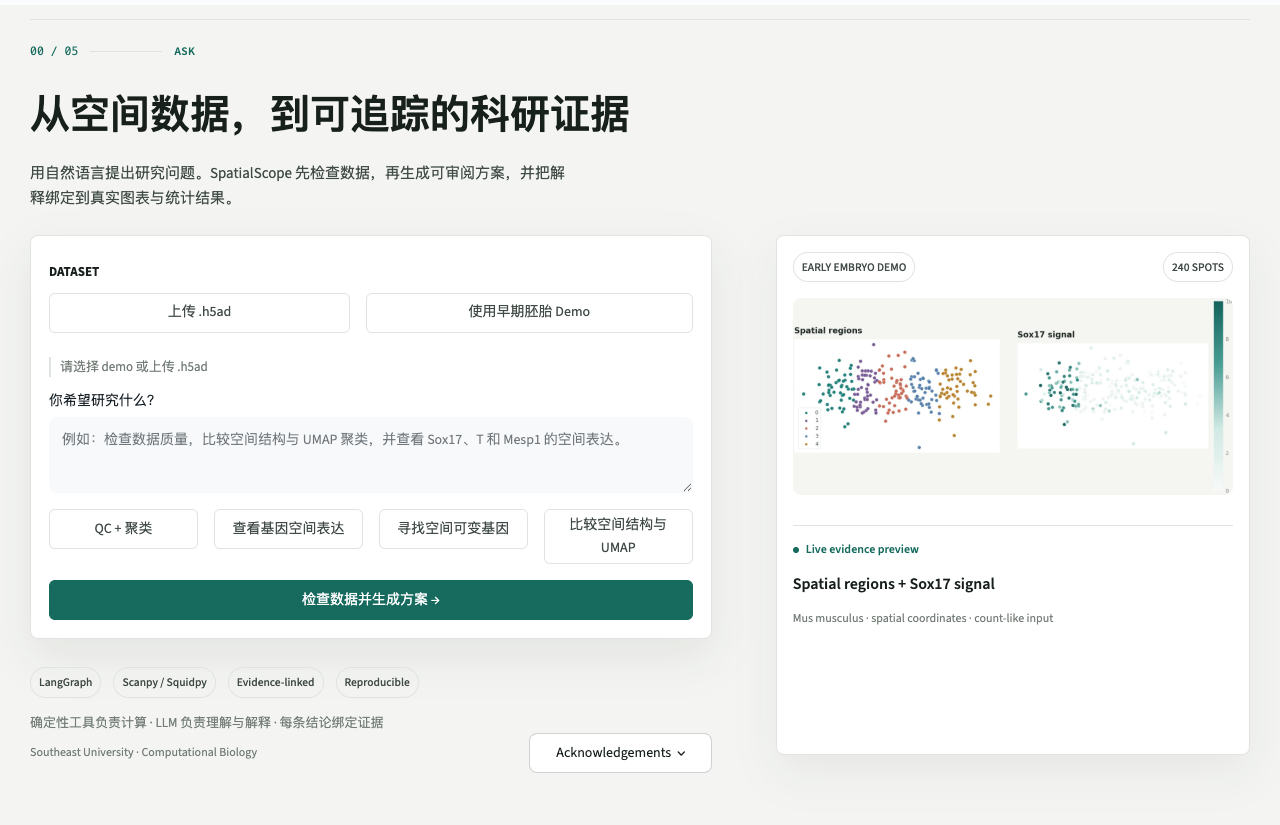
\includegraphics[width=0.92\textwidth]{assets/app_landing.png}\\[-0.2cm]
    {\small\color{scopeSlate}SpatialScope 主界面：中文界面、LLM 状态、Demo 入口与证据预览。}
  \end{center}
\end{titlepage}

\tableofcontents
\clearpage

\section*{摘要}
\addcontentsline{toc}{section}{摘要}

本项目围绕课程要求中的“空间转录组分析 Agent”展开，完成了一个可运行、可部署、
可审阅的交互式系统。系统以 LangGraph 组织 Agent 状态机，包含数据检查、自然语言
任务解析、分析计划生成、人工批准、工具执行、结果校验、修复、解释和报告生成等节点；
以 Scanpy/AnnData 为核心数据分析底座，支持 \code{.h5ad} 数据读取、质量控制、预处理、
PCA/UMAP/Leiden 聚类、空间可视化、基因空间表达和 marker gene 分析；以 OpenAI-compatible
LLM 接口接入 GLM 5.1，用于任务理解、研究简报、Copilot 问答和证据约束的解释生成。

系统设计避免将 Agent 简化为固定脚本或开放式聊天界面，而是采用“数据检查、计划生成、
工具执行、证据汇总、谨慎解释”的流程。最终报告与在线界面保留 evidence IDs、参数、图表、
trace、caveats 与可复现元数据；LLM 输出通过结构化 prompt、Pydantic schema 校验和 evidence
引用检查后才进入执行或报告链路。项目已上传 GitHub，并完成 Streamlit Cloud 在线部署。在线
demo 经浏览器端测试可完成选择数据、生成方案、批准运行、查看 Explore 和打开 Report 的完整流程；
本地测试通过 99 项单元测试，并在真实 GSE278603 E7.5 mouse embryo Stereo-seq 样本上完成
quick analysis smoke run。

\begin{summarybox}{交付状态}
  \begin{itemize}
    \item GitHub 仓库：\repoUrl
    \item 在线部署：\appUrl
    \item GitHub Pages 项目页：\pagesUrl
    \item 本地验证：\code{99 passed}；CLI smoke run 成功；线上 demo 完整流程成功。
    \item 真实数据验证：GSE278603 样本 \code{GSM9046244_Embryo_E7.5_stereo_rep2.h5ad}，
    8190 spots、16364 genes、空间坐标可用，quick run 0 warnings、0 errors。
  \end{itemize}
\end{summarybox}

\clearpage

\section{作业要求与完成情况}

课程任务明确要求使用 LangGraph 构建 Agent 核心流程，并实现空间转录组基础分析功能。
表 \ref{tab:requirement-map} 将作业要求与项目实现逐项对齐。整体判断是：基础要求已经完整
覆盖，扩展项中已完成在线部署、自动报告、交互式前端、空间可变基因/邻域分析接口与真实
数据示例；细胞通讯和高级模型作为后续路线图保留，暂不纳入 v1 主流程。

\begin{longtable}{L{0.27\textwidth}L{0.48\textwidth}L{0.17\textwidth}}
\caption{作业要求与 SpatialScope 实现映射。}\label{tab:requirement-map}\\
\toprule
作业要求 & 项目实现证据 & 状态 \\
\midrule
\endfirsthead
\toprule
作业要求 & 项目实现证据 & 状态 \\
\midrule
\endhead
LangGraph 核心框架 & \code{spatialscope/agent/graph.py}，Run 页面 live execution events，checkpointed plan review & 完成 \\
节点、边、状态、loop & inspect、parse、plan、review、execute、validate、repair、interpret、report 节点；失败修复与继续执行路径 & 完成 \\
Prompt / Tool / State / Workflow & LLM prompts、tool registry、Agent state、Quick/Standard/Advanced workflow & 完成 \\
自然语言输入 & Streamlit Project 输入框和 CLI \code{--query} & 完成 \\
\code{.h5ad} 读取与概览 & AnnData loader、dataset card、obs/var/obsm/layer schema preview & 完成 \\
QC 与预处理 & cell/gene 过滤、QC 图、normalize、log1p、HVG、scale & 完成 \\
PCA/UMAP/聚类 & PCA、neighbors、UMAP、Leiden 聚类和 cluster summary & 完成 \\
空间可视化 & cluster 空间图、gene 空间表达图、多基因 panel & 完成 \\
Marker gene 分析 & rank markers、marker table、marker heatmap & 完成 \\
结果解释 & Research Brief、evidence IDs、caveats、LLM guardrails & 完成 \\
自动报告 & HTML report、metadata、trace、parameters、bundle、报告页面 & 完成 \\
交互式前端 & Streamlit Project、Run、Explore、Report、Advanced & 完成 \\
在线部署 & Streamlit Cloud + GitHub Pages & 完成 \\
SVG / 邻域分析 & Squidpy 可选工具，未安装时 graceful fallback & 扩展完成 \\
细胞通讯 & 作为未来扩展，不放入 v1 主流程 & 未承诺 \\
\bottomrule
\end{longtable}

\section{设计原则：证据约束的 Agent 流程}

空间转录组分析不仅涉及 Scanpy 等工具的调用，还涉及数据对象、表达层、空间坐标字段、
聚类结果和图表解释之间的依赖关系。若缺少明确的状态管理、计划审阅、工具契约和证据边界，
Agent 容易退化为固定 notebook 或缺乏可复核性的对话界面。因此，本项目采用以下设计原则。

\begin{decisionbox}{原则一：先检查数据，再生成计划}
  Agent 在规划前读取 AnnData 的规模、obs/var 字段、obsm 空间坐标、raw/layer 状态和表达矩阵
  安全性。这样可以避免在不知道数据是否有空间坐标、是否有安全表达来源、基因是否存在的情况下
  直接解释结果。
\end{decisionbox}

\begin{decisionbox}{原则二：数值计算交给确定性工具，LLM 负责理解与叙述}
  LLM 不接触完整表达矩阵或完整空间坐标。它只接收 dataset summary、tool summary、figure/table
  metadata、warnings/errors 与 evidence pack。这一边界可以降低隐私、成本和幻觉风险。
\end{decisionbox}

\begin{decisionbox}{原则三：每条结论必须能回到证据}
  Report 与 Copilot 输出均绑定 evidence IDs。例如 \breakcode{execute_tool:plot_spatial:figure:0}
  和 \breakcode{gene:Pou5f1:summary}。该设计使解释能够回溯到图表、表格和工具输出，避免仅依赖
  不可追踪的自然语言结论。
\end{decisionbox}

\begin{decisionbox}{原则四：LLM 输出必须先结构化，再进入执行链路}
  LLM 的任务解析、方案生成、修复建议、finding 合成和 Copilot 回答均被要求返回 JSON，并经过
  Pydantic schema 校验。只有字段、类型和 evidence 引用符合预期的输出才会被 LangGraph 继续使用；
  校验失败时系统会回退到确定性规则或进入修复流程。
\end{decisionbox}

\begin{decisionbox}{原则五：主界面服务研究流程，底层审计进入 Advanced}
  主界面只保留 Project、Run、Explore、Report，避免把 tool registry、raw JSON、audit score
  等低层信息堆在用户面前。高级 provenance 信息集中到 Advanced 区域，供复核和调试。
\end{decisionbox}

\section{系统架构}

\subsection{LangGraph 工作流}

图 \ref{fig:architecture} 展示了 SpatialScope 的核心 Agent 流程。该流程并非单次函数调用，
而是可中断、可恢复、可校验、可修复的状态机。用户问题进入系统后，Agent 先检查数据，再将自然语言
转成 ResearchBrief 和分析计划。计划展示给用户审阅，批准后才执行工具。每个工具执行后进入
validate 节点；如果失败或参数不安全，repair 节点会尝试修正或要求 clarification。最终，系统
基于工具产物生成报告和 Copilot 可用的 evidence pack。

\begin{figure}[H]
\centering
\resizebox{\textwidth}{!}{%
\begin{tikzpicture}[
  x=1cm,
  y=1cm,
  main/.style={rounded corners=2mm, draw=scopeTeal!92!black, fill=scopeMist, line width=0.75pt,
    align=center, minimum width=2.35cm, minimum height=1.00cm, font=\small},
  review/.style={rounded corners=2mm, draw=scopeGold!85!black, fill=scopeGold!13, line width=0.75pt,
    align=center, minimum width=2.35cm, minimum height=1.00cm, font=\small},
  support/.style={rounded corners=2mm, draw=scopeBlue!80!black, fill=scopeBlue!6, line width=0.7pt,
    align=center, minimum height=0.82cm, font=\small},
  statebox/.style={rounded corners=2mm, draw=scopeSlate!80!black, fill=scopeSlate!7, line width=0.7pt,
    align=center, minimum height=0.82cm, font=\small},
  arrow/.style={-{Stealth[length=2.3mm,width=1.8mm]}, line width=0.8pt, draw=scopeTeal!90!black},
  looparrow/.style={-{Stealth[length=2.3mm,width=1.8mm]}, line width=0.8pt, draw=scopeGold!85!black},
  softarrow/.style={-{Stealth[length=2.0mm,width=1.5mm]}, dashed, line width=0.65pt, draw=scopeBlue!80!black}
]
\node[main] (inspect) at (0,0) {输入与检查\\问题 + AnnData};
\node[main] (parse) at (2.50,0) {任务解析\\ResearchBrief};
\node[review] (plan) at (5.00,0) {方案审阅\\人工批准};
\node[main] (execute) at (7.50,0) {工具执行\\QC / UMAP};
\node[review] (validate) at (10.00,0) {校验修复\\安全检查};
\node[main] (report) at (12.50,0) {证据报告\\Explore / Report};

\node[support, minimum width=6.20cm] (llm) at (3.75,1.55) {LLM 支持模块（GLM 5.1）\\理解问题、补全计划、生成证据约束解释};
\node[support, minimum width=4.70cm] (tools) at (7.50,-1.75) {确定性工具层\\Scanpy / AnnData / 图表生成};
\node[statebox, minimum width=4.95cm] (state) at (11.25,1.55) {状态与证据层\\trace、metadata、parameters、evidence IDs};

\draw[arrow] (inspect) -- (parse);
\draw[arrow] (parse) -- (plan);
\draw[arrow] (plan) -- (execute);
\draw[arrow] (execute) -- (validate);
\draw[arrow] (validate) -- (report);

\draw[looparrow] (validate.south) |- node[pos=0.22,right,font=\scriptsize,color=scopeGold!85!black]{失败或不安全} ([yshift=-0.95cm]validate.south) -| (execute.south);

\draw[softarrow] (llm.south west) -- (parse.north);
\draw[softarrow] (llm.south) -- (plan.north);
\draw[softarrow] (tools.north) -- (execute.south);
\draw[softarrow] (state.south west) -- (validate.north);
\draw[softarrow] (state.south east) -- (report.north);
\end{tikzpicture}
}
\caption{SpatialScope Agent 的 LangGraph 架构。主流程从输入与数据检查开始，经过任务解析、方案生成与人工审阅后进入确定性工具执行；校验失败或表达层不安全时回到工具执行前进行修复；LLM、工具层和状态证据层分别承担理解、计算和可复核记录。}
\label{fig:architecture}
\end{figure}

\subsection{状态设计}

Agent state 中保留 \code{run_id}、\code{dataset_hash}、\code{task_plan}、\code{approved_plan}、
parameters、figures、tables、warnings、errors、environment 和 \code{execution_trace}。大型
AnnData 对象不进入公共状态，而是以工作副本和摘要形式管理。这个选择有三个好处：

\begin{itemize}
  \item 降低 Streamlit session 与 LLM context 的负担；
  \item 保证报告和 trace 可以安全分享；
  \item 让每个 run 都能独立复核、下载和复跑。
\end{itemize}

\subsection{工具契约}

工具层按照“输入前置条件、输出后置条件、常见失败、修复策略”组织。核心工具包括：

\begin{itemize}
  \item IO：读取 \code{.h5ad}、识别空间坐标别名、生成 dataset profile。
  \item QC：计算 total counts、detected genes、mitochondrial fraction 与过滤摘要。
  \item Preprocess：建立 expression lineage，生成 interpretation layer 与 modeling representation。
  \item Clustering：PCA、neighbors、UMAP、Leiden。
  \item Spatial plots：cluster 空间图、gene panel、linked Explore evidence。
  \item Marker genes：rank genes groups、top markers、marker heatmap。
  \item Report：HTML report、trace、metadata、artifact manifest、run bundle。
\end{itemize}

\section{LLM 设计与安全边界}

项目使用 OpenAI-compatible 接口接入 GLM 5.1。LLM 不承担数值分析角色，而是在以下边界内参与任务理解和解释：

\begin{table}[H]
\centering
\caption{LLM 在 SpatialScope 中的职责边界。}
\begin{tabularx}{\textwidth}{L{0.22\textwidth}Y}
\toprule
允许 LLM 做 & 不允许 LLM 做 \\
\midrule
解析自然语言任务，生成 ResearchBrief & 读取完整表达矩阵或完整空间坐标 \\
根据数据摘要建议分析计划 & 替代 Scanpy/Squidpy 数值计算 \\
基于 evidence pack 回答 Copilot 问题 & 在没有 evidence IDs 时生成最终结论 \\
把工具摘要写成谨慎解释 & 编造细胞类型、发育机制或因果解释 \\
\bottomrule
\end{tabularx}
\end{table}

这条边界尤其重要。空间组学数据常常维度高、样本大、解释敏感。如果把原始矩阵直接交给 LLM，
不仅成本高，也会削弱结果的可复现性。SpatialScope 的做法是：工具先产生可追踪证据，LLM 只能围绕
证据组织语言。

\subsection{Prompt 结构、Evidence IDs 与 Schema 校验}

SpatialScope 的 prompt 不是一个开放式聊天模板，而是分布在 Agent 不同阶段的结构化指令。系统 prompt
首先规定模型必须基于 evidence pack 回答，不能请求完整表达矩阵或原始空间坐标，不能编造基因、细胞类型、
\emph{p}-value 或机制结论；随后每个节点再提供对应 schema，让 LLM 输出可被程序验证的 JSON。

\begin{table}[H]
\centering
\caption{LLM prompt 在 Agent 流程中的作用。}
\begin{tabularx}{\textwidth}{L{0.22\textwidth}L{0.27\textwidth}Y}
\toprule
阶段 & 结构化输出 & 作用 \\
\midrule
任务解析 & \code{ResearchBrief} & 从自然语言中提取目标、基因、约束和需要澄清的问题。 \\
方案生成 & \code{V2AnalysisPlan} & 根据数据概况和工具契约生成可审阅、可执行的步骤。 \\
失败修复 & \code{RepairDecision} & 对缺失基因、错误参数或不安全表达层给出有边界的修复建议。 \\
结果合成 & \code{ScientificFinding[]} & 从 evidence packs 中生成 3--5 条带证据和局限的 finding。 \\
Explore 问答 & \code{CopilotAnswer} & 基于当前 Spatial / UMAP / gene / cluster 选择回答问题，并列出证据编号。 \\
\bottomrule
\end{tabularx}
\end{table}

Evidence ID 是系统为每个图、表、指标或交互式摘要生成的证据编号。例如
\breakcode{execute_tool:plot_umap:figure:0} 指向 UMAP 图，
\breakcode{execute_tool:rank_markers:table:0} 指向 marker 表格，
\breakcode{gene:Sox17:summary} 指向 Explore 页面中 Sox17 的当前统计摘要。LLM 在生成 finding
或 Copilot 回答时必须返回使用过的 exact evidence IDs；报告端会把这些编号显示出来，方便用户从一句
解释反查到具体图表和工具输出。

Schema 校验则把 LLM 输出从自然语言建议变成程序可执行的对象。实现中，LLM 返回的 JSON 会经过
\code{ResearchBrief.model_validate}、\code{V2AnalysisPlan.model_validate}、
\code{RepairDecision.model_validate} 或 \code{ScientificFinding.model_validate} 等 Pydantic
校验；分析计划还会再经过工具注册表校验，确保 \code{tool} 名称真实存在、参数结构可读。对于报告
finding，系统还会检查其 \code{evidence_ids} 是否真的存在于当前 run 的 evidence packs 中。如果
LLM 输出格式错误、引用了不存在的证据，或 evidence-grounded findings 数量不足，系统不会强行采纳，
而是记录 telemetry 并切换到确定性 fallback。

\begin{table}[H]
\centering
\caption{Evidence 与 schema 机制解决的主要风险。}
\begin{tabularx}{\textwidth}{L{0.24\textwidth}Y Y}
\toprule
机制 & 具体实现 & 降低的风险 \\
\midrule
Evidence IDs & 图、表、metric 和 Explore 摘要统一编号，Report 与 Copilot 显示 exact IDs。 &
避免结论无法追踪，减少“只看起来合理”的解释。 \\
EvidencePack & 只向 LLM 提供标题、caption、summary metrics、少量表格摘录和 caveats。 &
避免传入原始矩阵，降低隐私、上下文长度和成本风险。 \\
Schema validation & LLM 输出必须通过 Pydantic 模型和工具注册表校验。 &
避免把随意文本或不存在的工具步骤交给执行器。 \\
Fallback and guardrails & 校验失败、证据不足或数值问题时使用规则 fallback 和谨慎措辞。 &
避免模型在证据不足时生成过度确定的生物学结论。 \\
\bottomrule
\end{tabularx}
\end{table}

\section{产品界面与交互流程}

\subsection{Project：从问题到数据理解}

Project 页面是用户进入系统的第一步。用户可以上传 \code{.h5ad} 或使用早期胚胎 demo，并用自然
语言提出问题。系统会先检查数据，而不是立即运行脚本。图 \ref{fig:project-flow} 显示了 Project
阶段的两个状态：初始入口和数据理解结果。

\begin{figure}[H]
\centering
\begin{subfigure}{0.49\textwidth}
  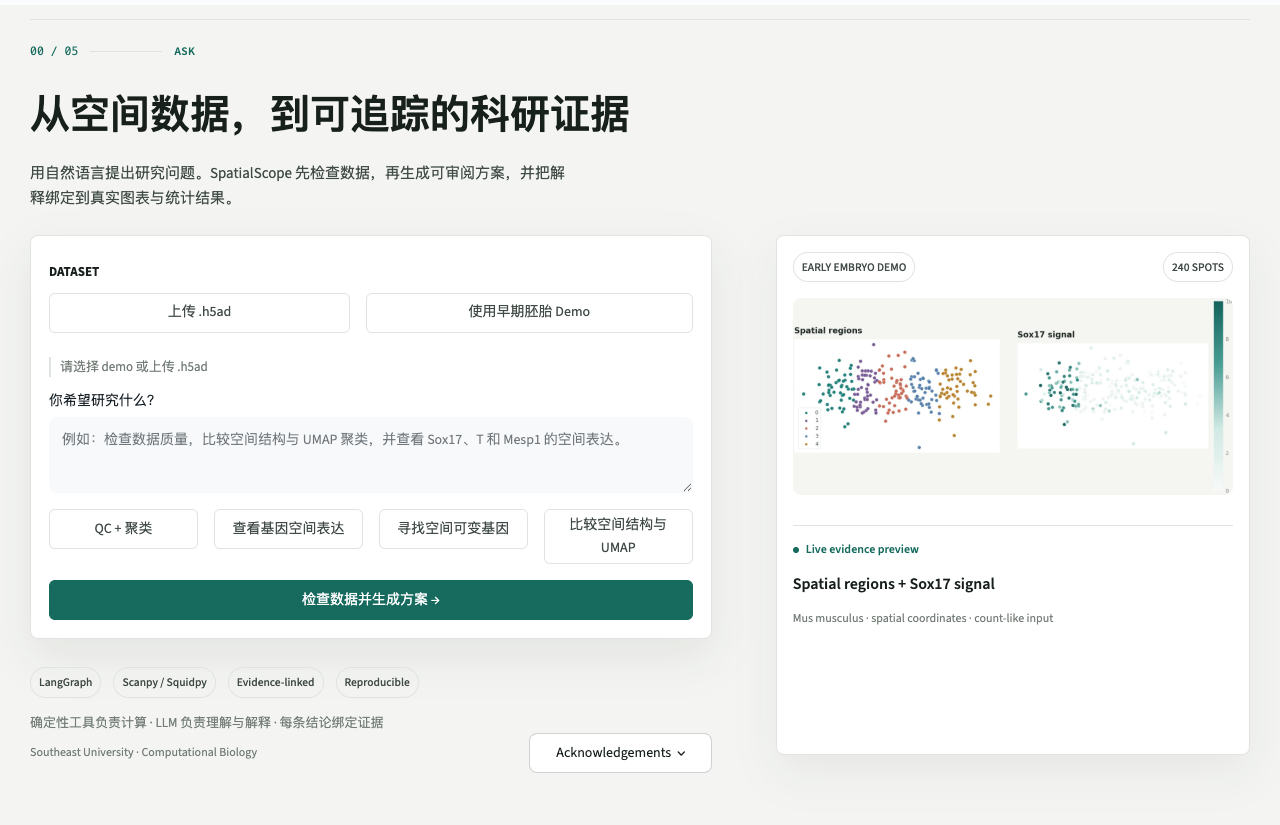
\includegraphics[width=\linewidth]{assets/app_landing.png}
  \caption{项目入口：自然语言问题、demo 数据、LLM 状态和视觉签名。}
\end{subfigure}
\hfill
\begin{subfigure}{0.49\textwidth}
  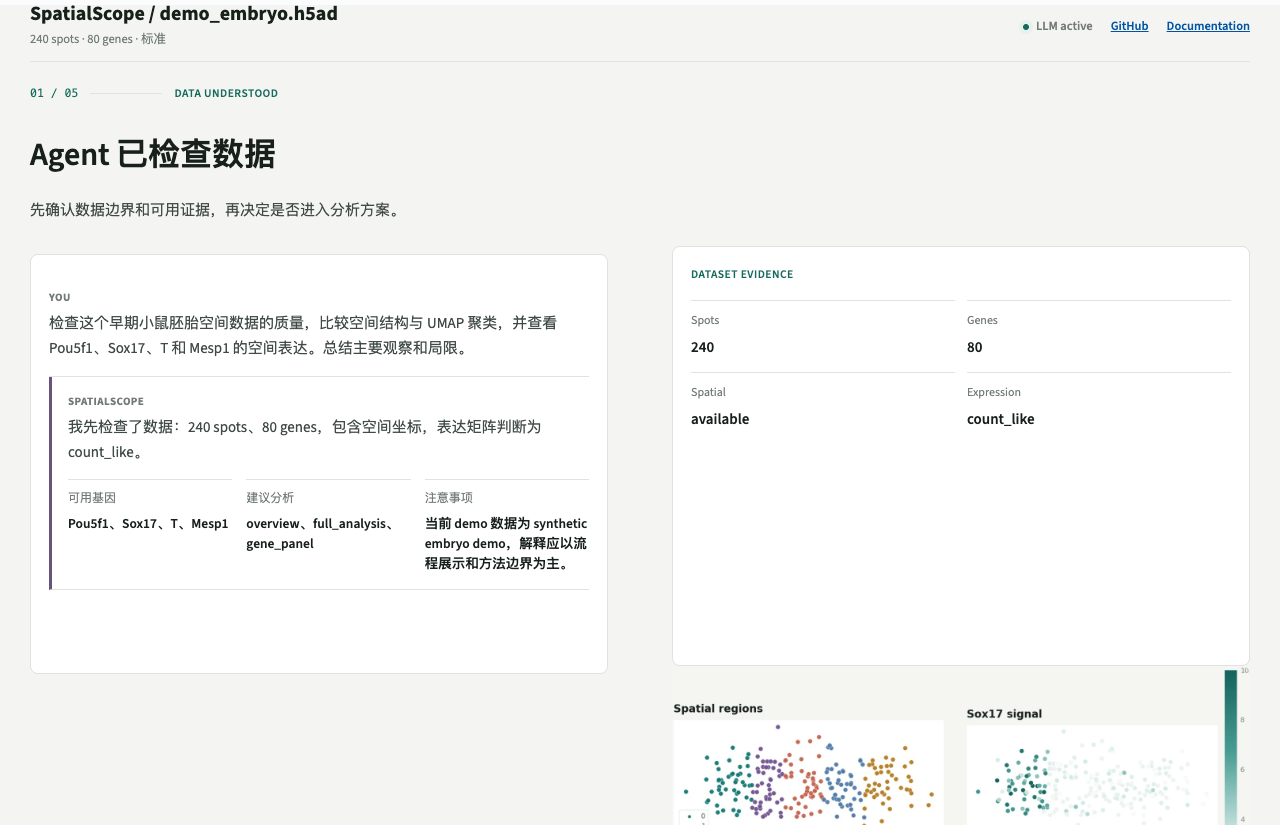
\includegraphics[width=\linewidth]{assets/app_dataset_understood.png}
  \caption{数据理解：spots、genes、空间坐标和表达矩阵状态。}
\end{subfigure}
\caption{Project 页面体现“先理解数据，再制定计划”的交互原则。}
\label{fig:project-flow}
\end{figure}

\subsection{Plan Review 与 Run：Human-in-the-loop}

用户批准前，Agent 会把分析方案展示为“分析契约”：每一步的目的、参数和预期产物都可见。批准后，
Run 页面以 live events 展示 LangGraph 节点进度。该设计用于呈现 Agent 的执行状态、工具参数和产物数量，
减少对单一阻塞状态提示的依赖。

\begin{figure}[H]
\centering
\begin{subfigure}{0.49\textwidth}
  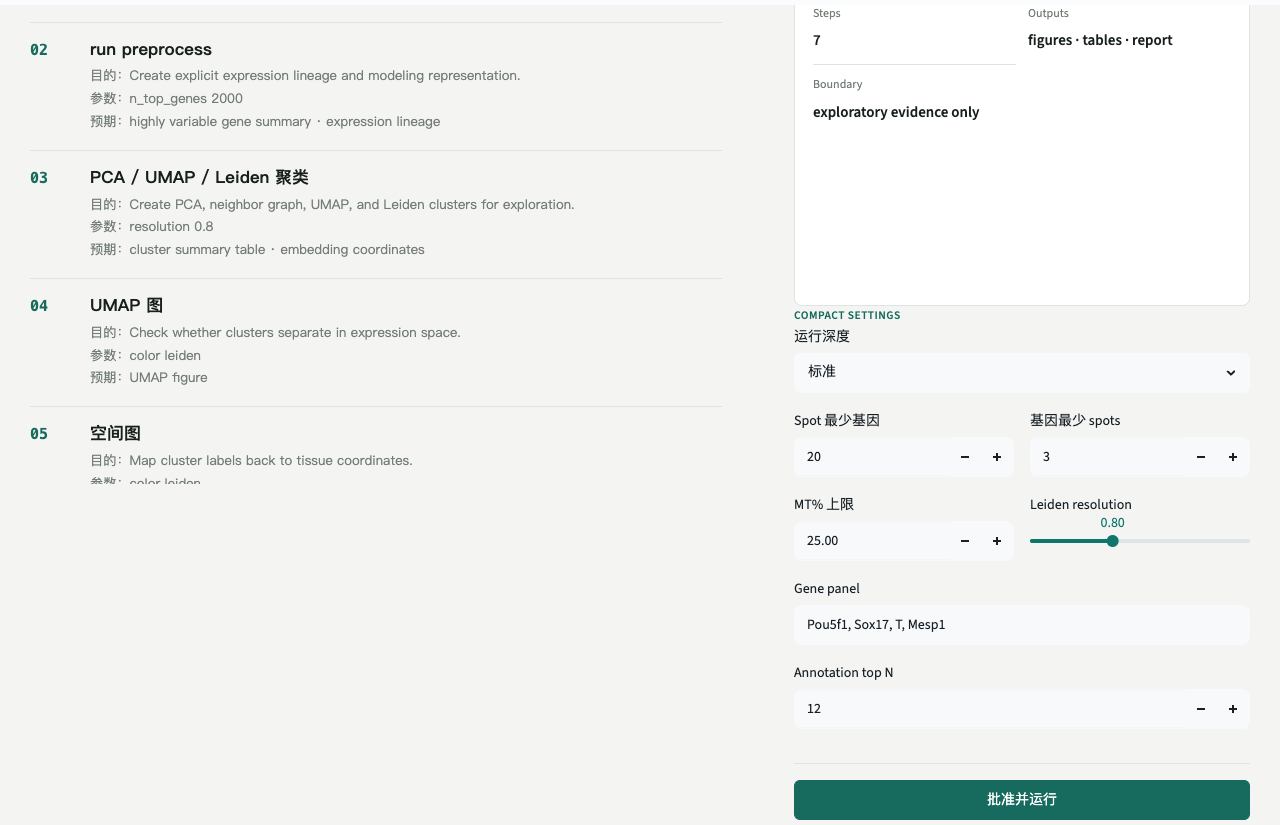
\includegraphics[width=\linewidth]{assets/app_plan_review.png}
  \caption{Plan Review：7 步标准分析方案和可调参数。}
\end{subfigure}
\hfill
\begin{subfigure}{0.49\textwidth}
  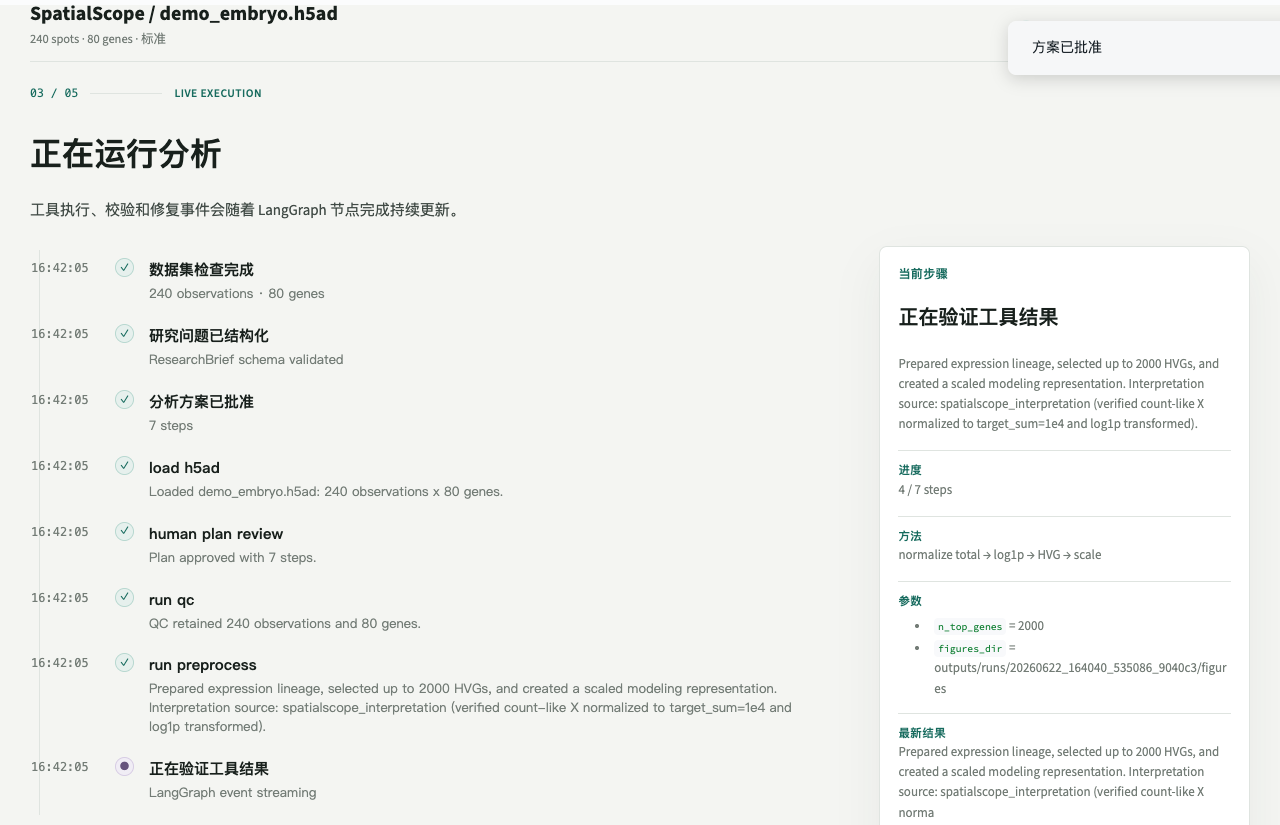
\includegraphics[width=\linewidth]{assets/app_run_live.png}
  \caption{Run：LangGraph 事件流、当前工具、参数和产物数量。}
\end{subfigure}
\caption{从计划批准到实时执行的 human-in-the-loop 流程。}
\label{fig:plan-run}
\end{figure}

\subsection{Explore 与 Report：证据优先}

Explore 页面把 Spatial 与 UMAP 并排展示，共享 cluster palette，并提供基因、cluster、表达层和
percentile clipping 控件。Copilot 回答必须显示使用的 evidence IDs。Report 页面则把 3-5 条
finding、quantitative support、evidence IDs 与 caveats 组织成可审阅的 Research Brief。

\begin{figure}[H]
\centering
\begin{subfigure}{0.49\textwidth}
  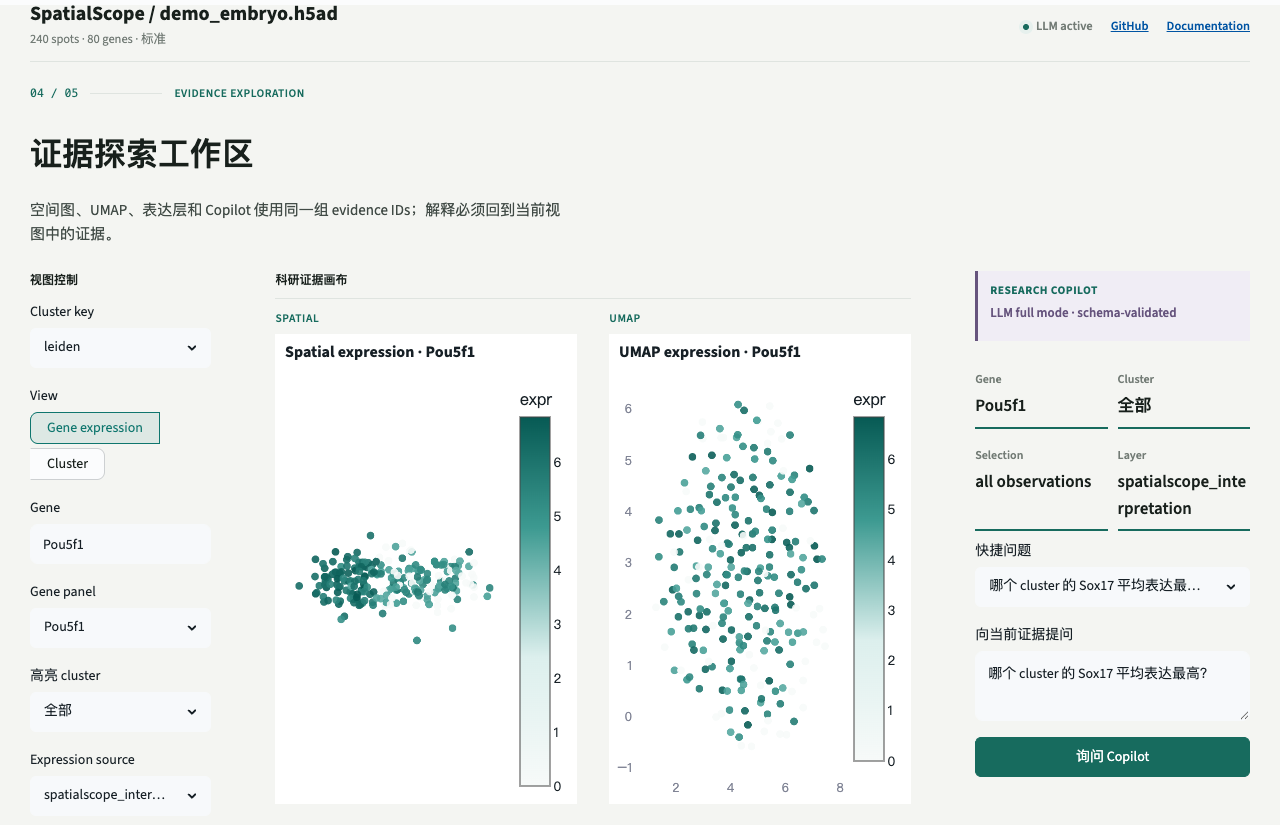
\includegraphics[width=\linewidth]{assets/app_explore.png}
  \caption{Explore：Spatial + UMAP 联动，Copilot 绑定当前 evidence。}
\end{subfigure}
\hfill
\begin{subfigure}{0.49\textwidth}
  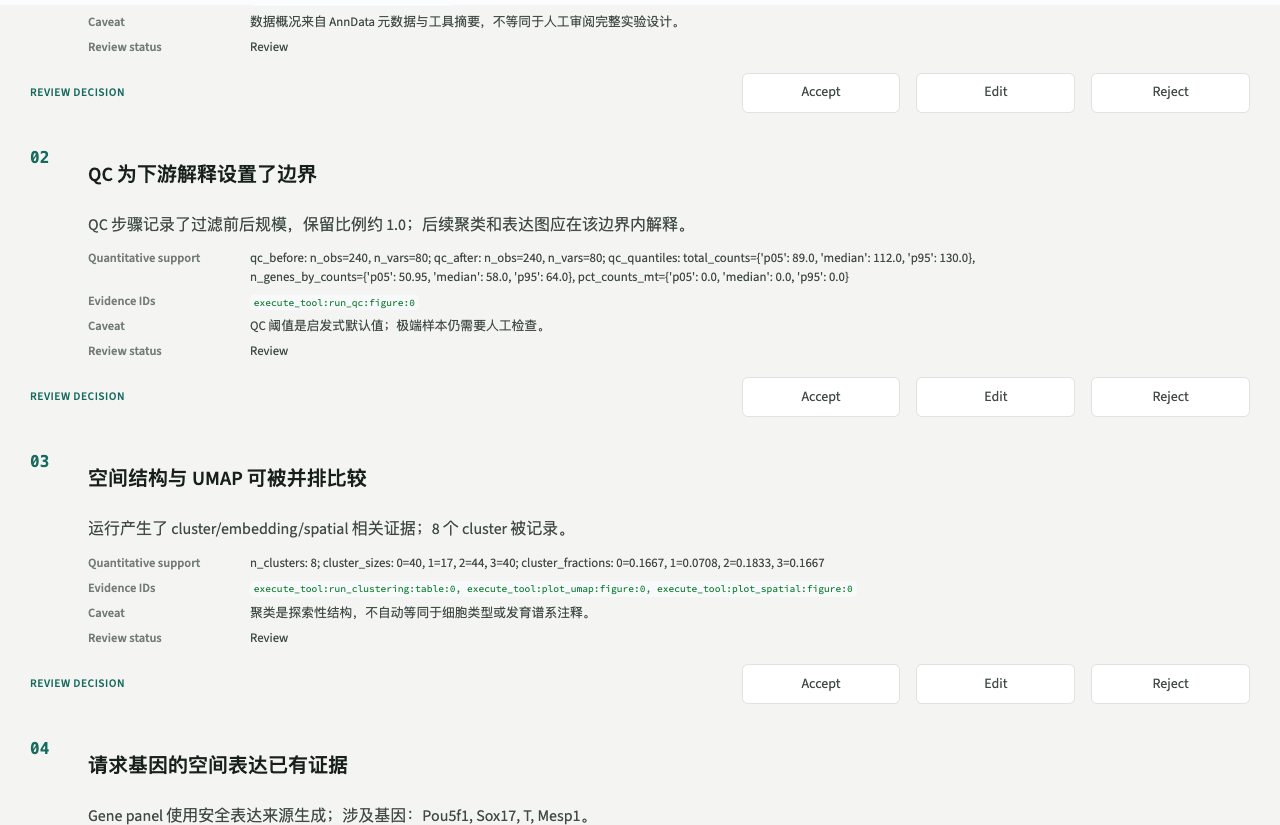
\includegraphics[width=\linewidth]{assets/app_report.png}
  \caption{Report：finding、证据、局限和 primary visual evidence。}
\end{subfigure}
\caption{主展示页面强调证据、可视化和谨慎解释。}
\label{fig:explore-report}
\end{figure}

\section{空间转录组分析功能实现}

SpatialScope 当前支持三种运行深度：Quick、Standard、Advanced。Quick 适合快速验证数据和图表；
Standard 完整覆盖课程要求的 QC、preprocess、UMAP/Leiden、空间图、gene panel、marker gene 和
report；Advanced 在 Standard 基础上尝试 SVG 和 neighborhood enrichment，如果 Squidpy 不可用则
记录结构化 warning 而不是崩溃。

\begin{table}[H]
\centering
\caption{三种运行模式的功能边界。}
\begin{tabularx}{\textwidth}{L{0.18\textwidth}Y}
\toprule
模式 & 内容 \\
\midrule
Quick & 数据检查、QC 摘要、预处理、UMAP/Leiden、空间 cluster 图、gene panel、简要报告。 \\
Standard & Quick + marker gene ranking、marker heatmap、完整 Research Brief、dataset card、trace、bundle。 \\
Advanced & Standard + SVG 和空间邻域分析扩展；依赖 Squidpy 时启用，缺失时 graceful fallback。 \\
\bottomrule
\end{tabularx}
\end{table}

实现中重点处理了表达来源安全问题。对于 count-like \code{X}，系统会生成归一化和 log1p 的
\code{spatialscope_interpretation} 作为解释层；对于未知或 scaled \code{X}，如果没有安全 raw/layer，
marker 和 gene interpretation 会被阻断或要求 clarification。这一点是为了避免在错误表达层上生成
看似合理但科学上不可靠的解释。

\section{Demo 结果与浏览器端验收}

\subsection{标准 demo run}

在线 demo 使用 synthetic early embryo spatial dataset，包含 Pou5f1、Sox17、T、Mesp1 等早期胚胎
相关基因。该数据集主要用于展示流程，不声称产生真实生物学发现。一次 Standard run 的摘要如下：

\begin{table}[H]
\centering
\caption{标准 demo run 的产物摘要。}
\begin{tabularx}{\textwidth}{L{0.28\textwidth}Y}
\toprule
项目 & 数值 \\
\midrule
Run ID & \code{20260622_165428_671120_e91308} \\
数据规模 & 240 spots，80 genes，空间坐标可用 \\
表达矩阵状态 & count-like；系统生成安全 interpretation layer \\
分析计划 & 7 步标准流程 \\
执行 trace & 10 events \\
产物 & 6 figures，4 tables，\code{report.html}，\code{agent_trace.json}，\code{run_metadata.json} \\
Warnings / Errors & 0 / 0 \\
\bottomrule
\end{tabularx}
\end{table}

\begin{figure}[H]
\centering
\begin{subfigure}{0.49\textwidth}
  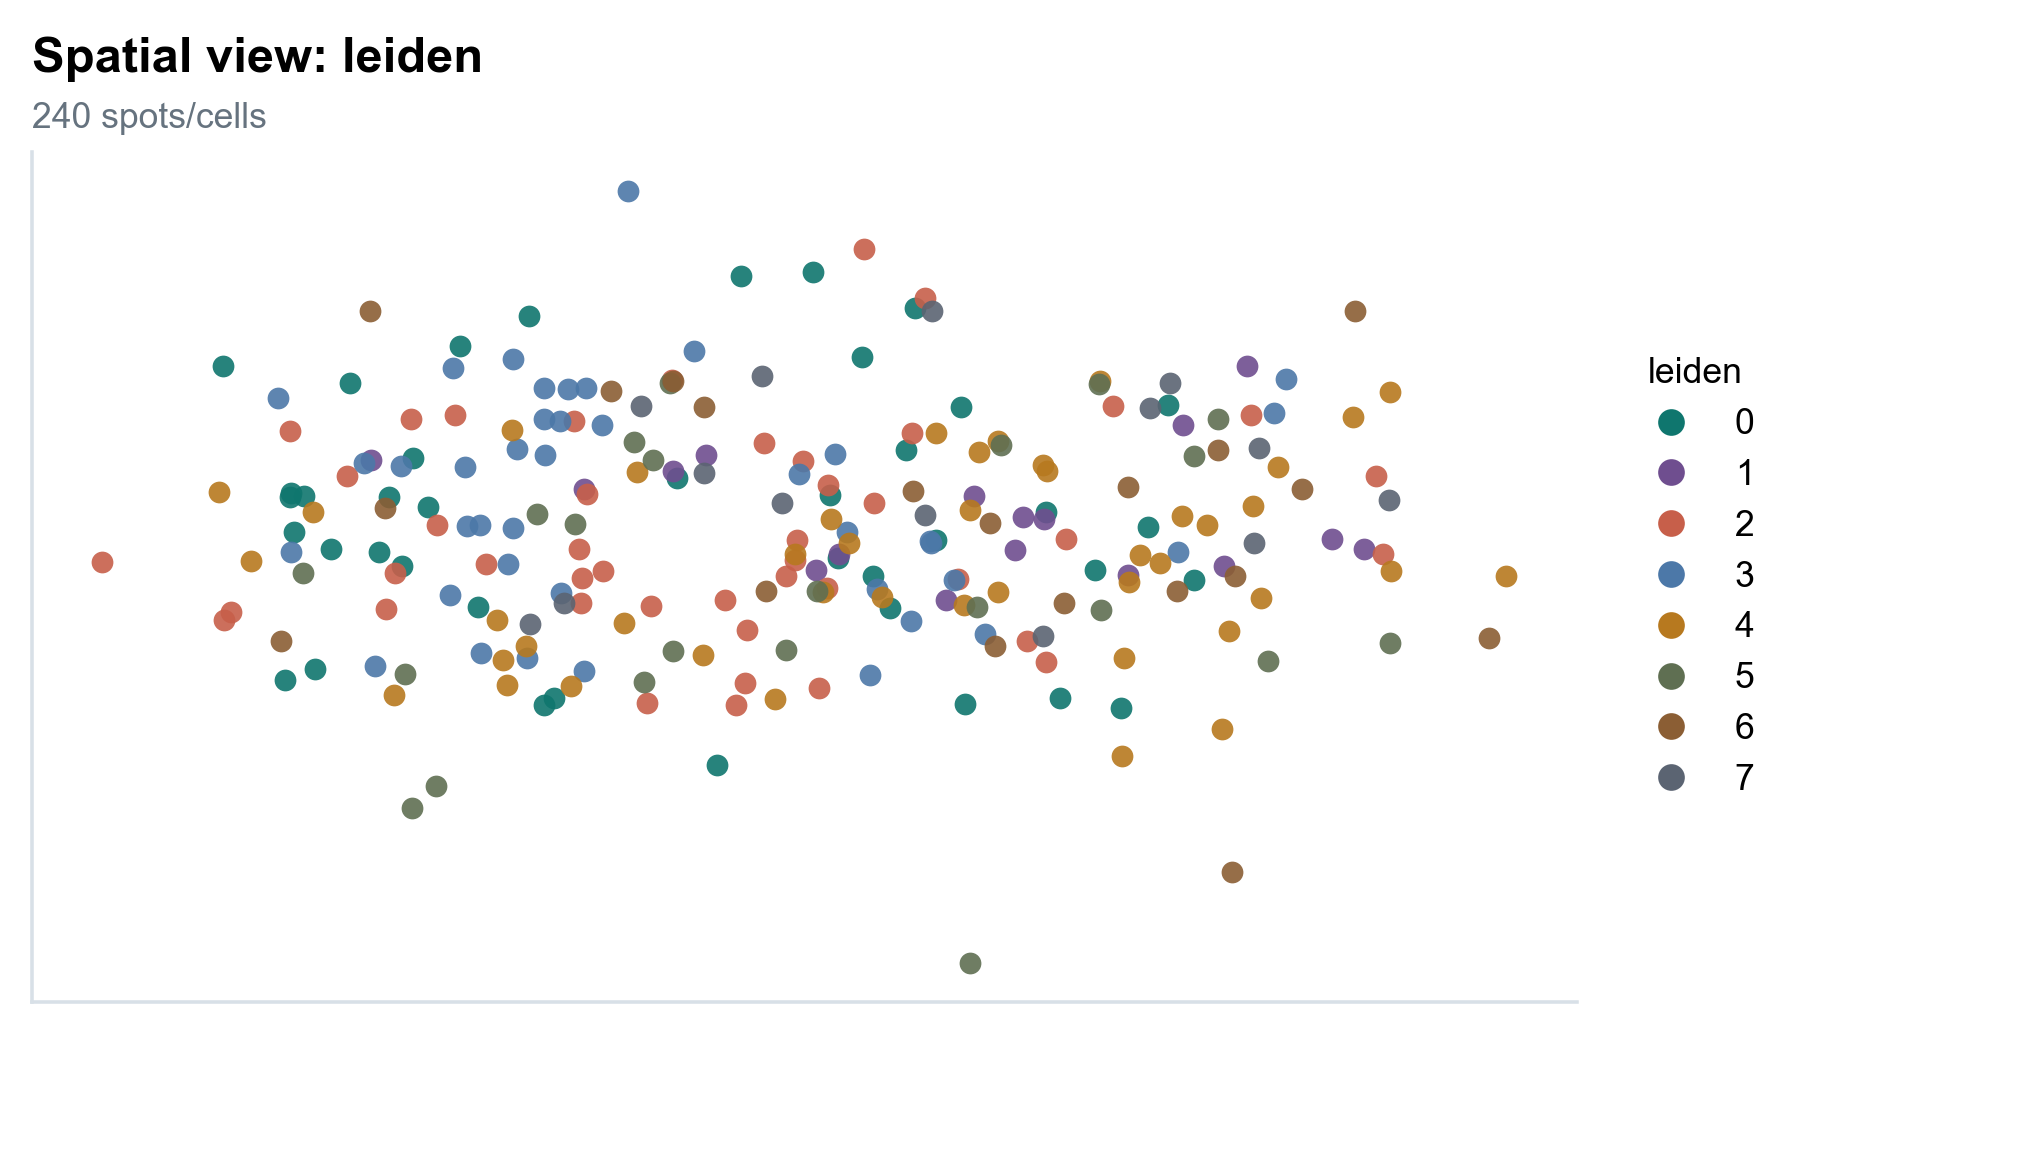
\includegraphics[width=\linewidth]{assets/demo_spatial_leiden.png}
  \caption{Leiden cluster 的空间分布。}
\end{subfigure}
\hfill
\begin{subfigure}{0.49\textwidth}
  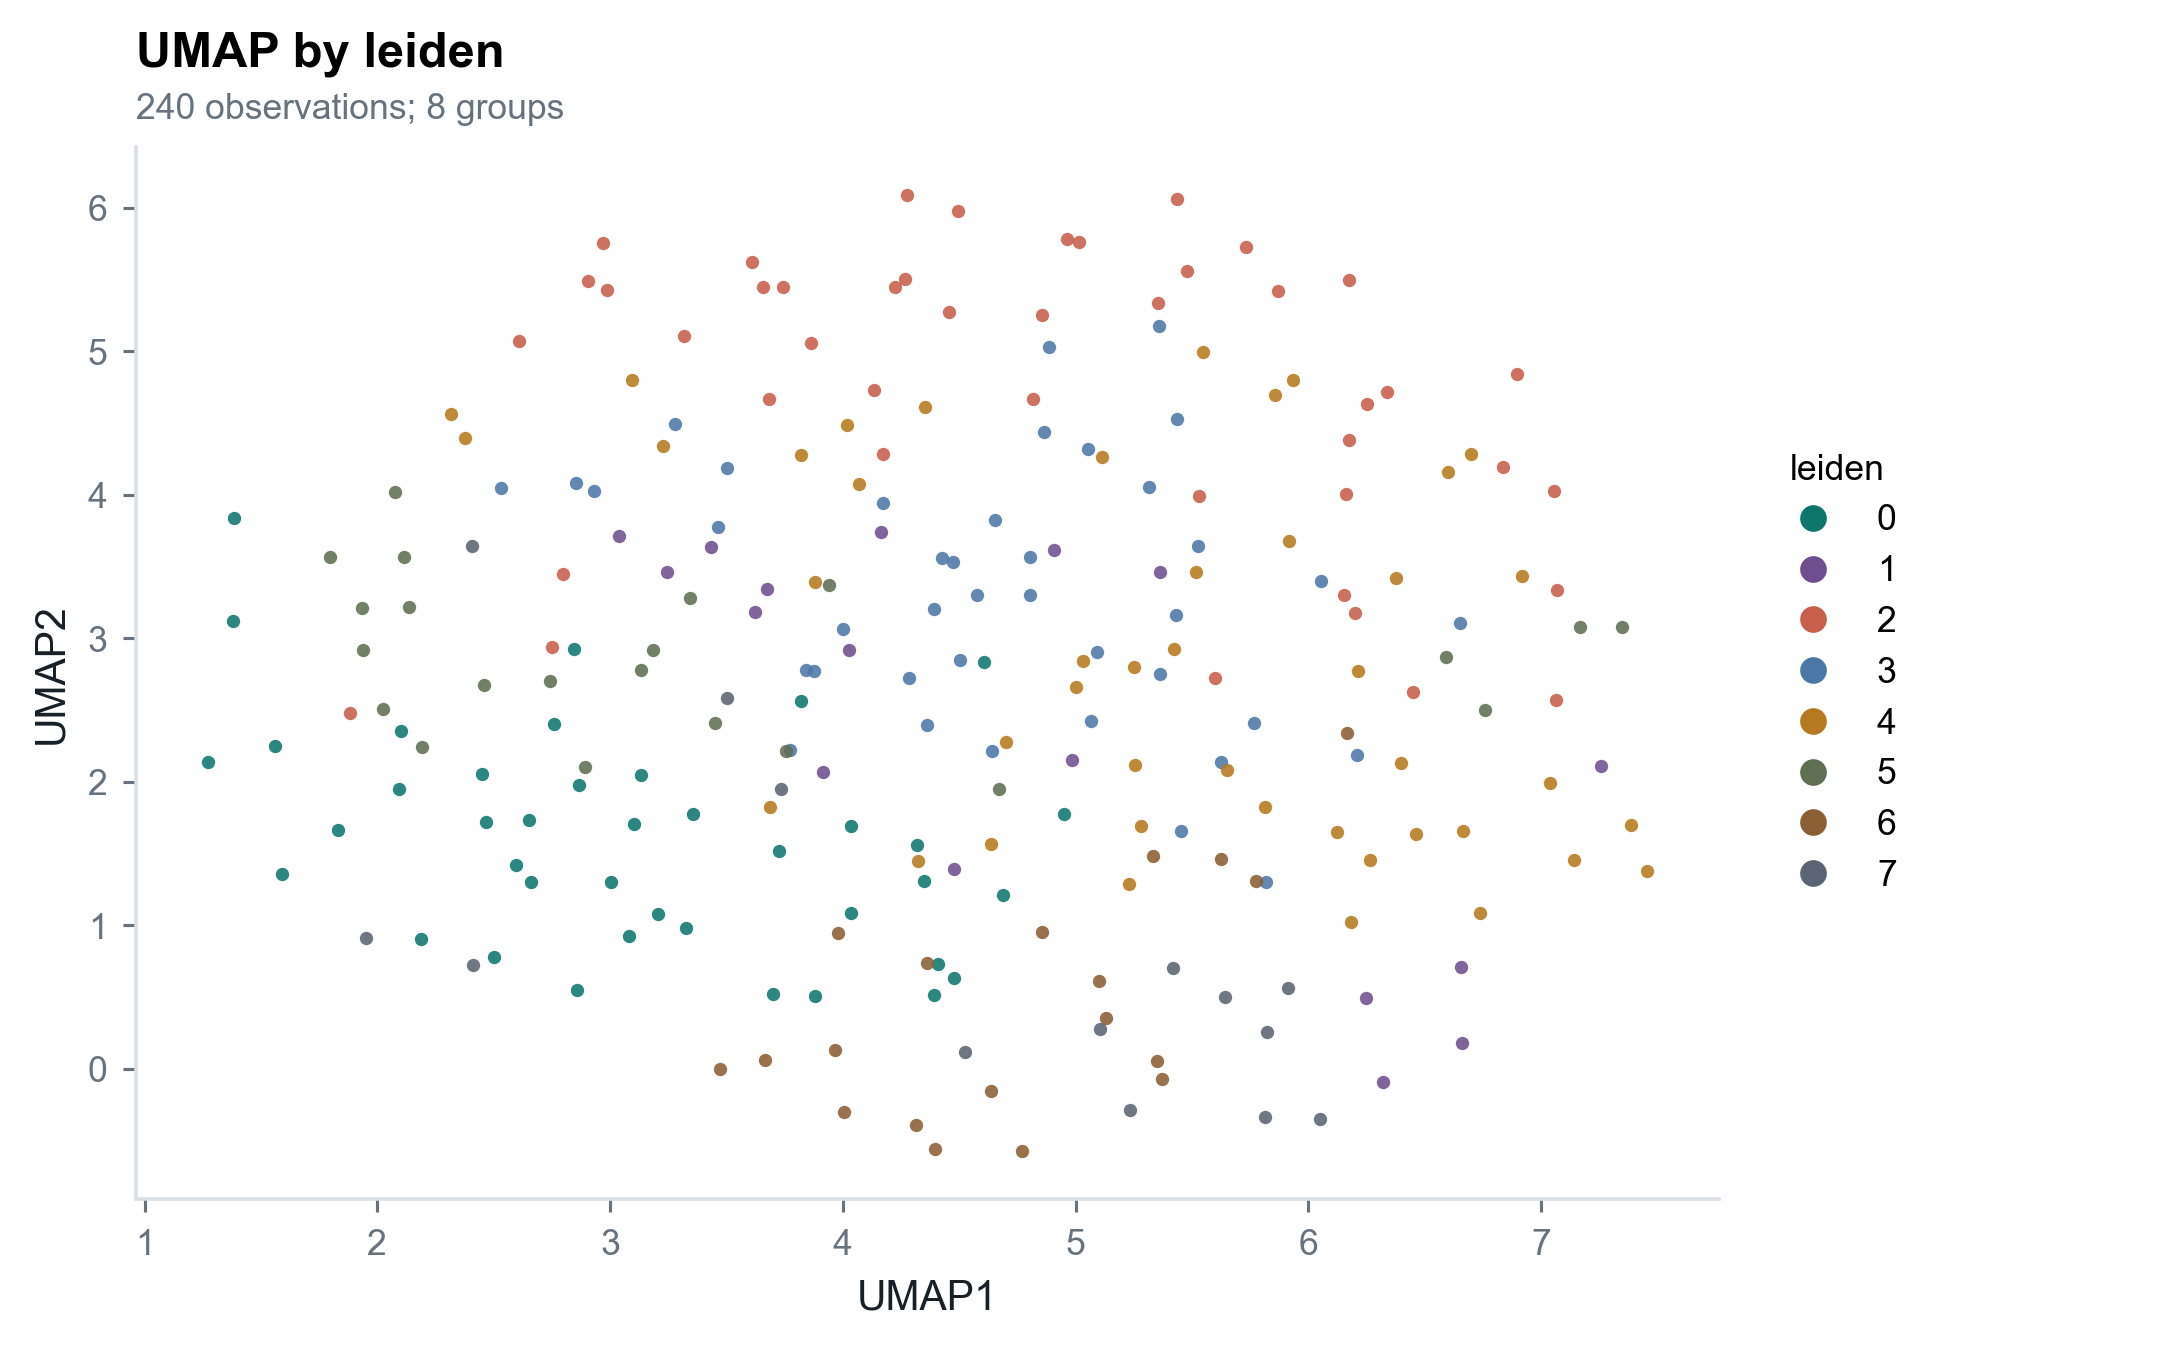
\includegraphics[width=\linewidth]{assets/demo_umap_leiden.png}
  \caption{UMAP 中的 cluster 分离。}
\end{subfigure}
\caption{标准 demo 的空间结构与表达空间结构对照。}
\label{fig:demo-cluster}
\end{figure}

\begin{figure}[H]
\centering
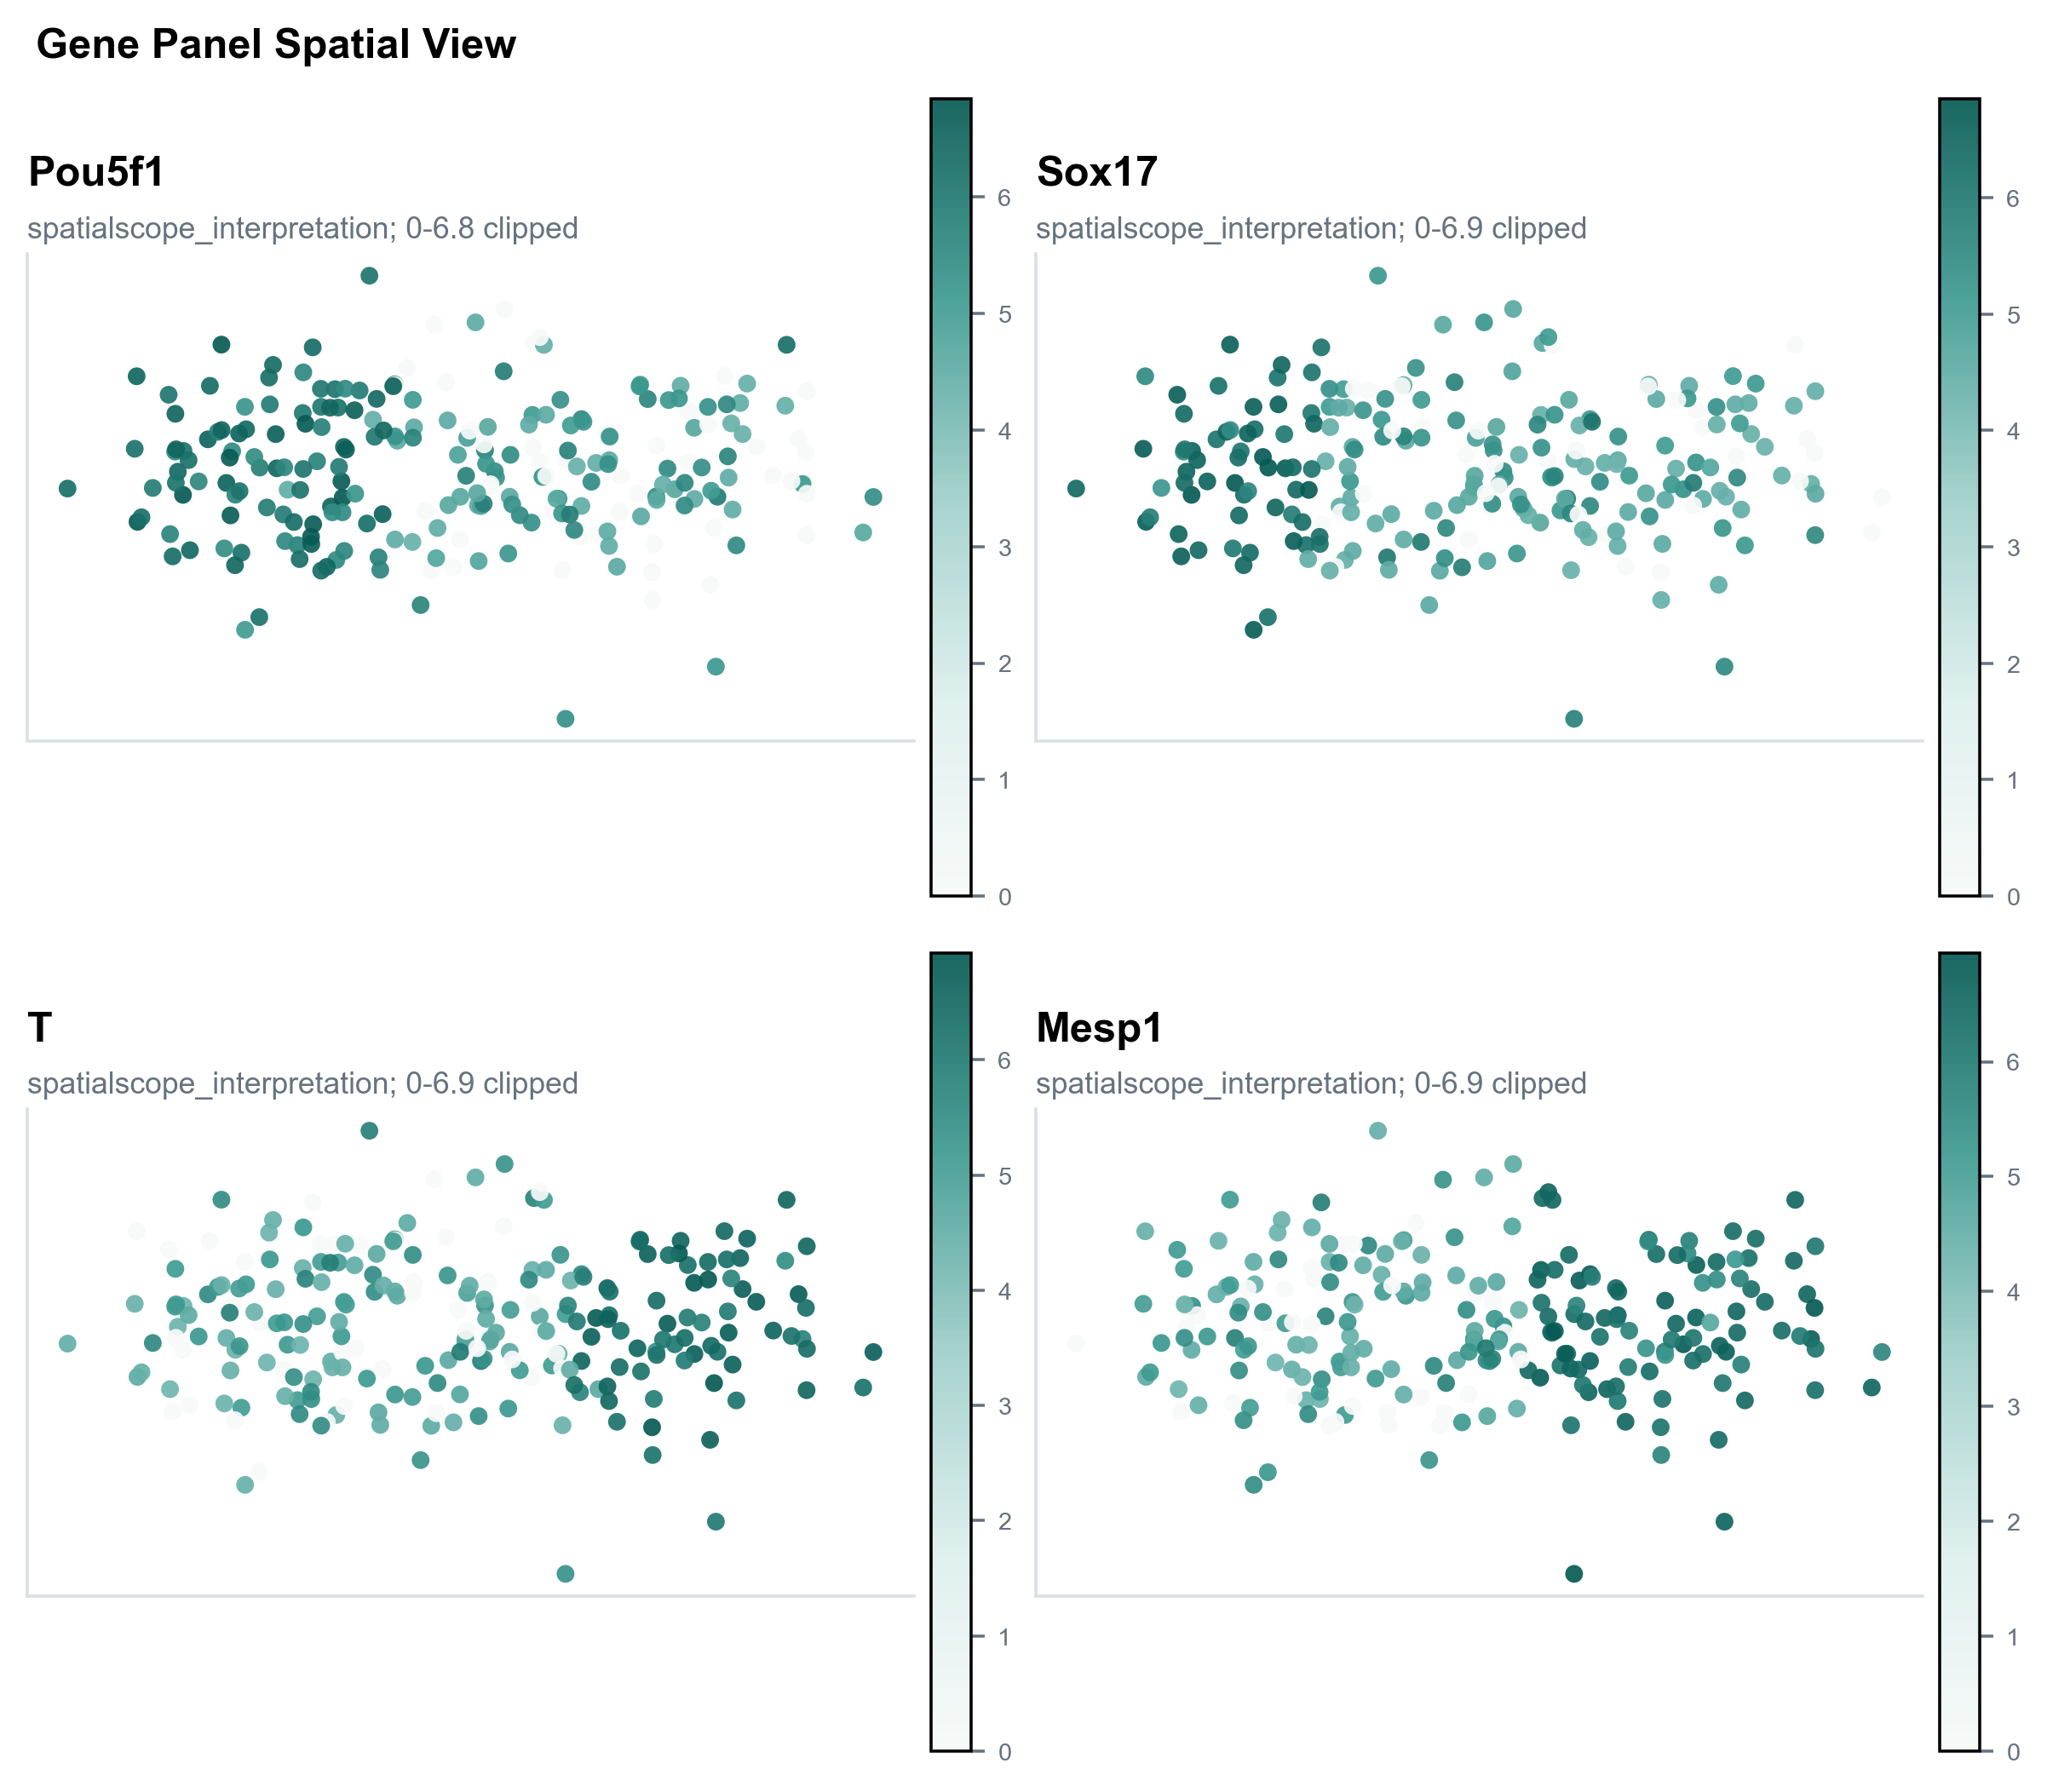
\includegraphics[width=0.96\textwidth]{assets/demo_gene_panel.png}
\caption{请求基因 Pou5f1、Sox17、T、Mesp1 的空间表达 panel。图表只作为 demo 数据上的流程展示，不被解释为真实生物学发现。}
\label{fig:demo-gene-panel}
\end{figure}

\begin{figure}[H]
\centering
\begin{subfigure}{0.49\textwidth}
  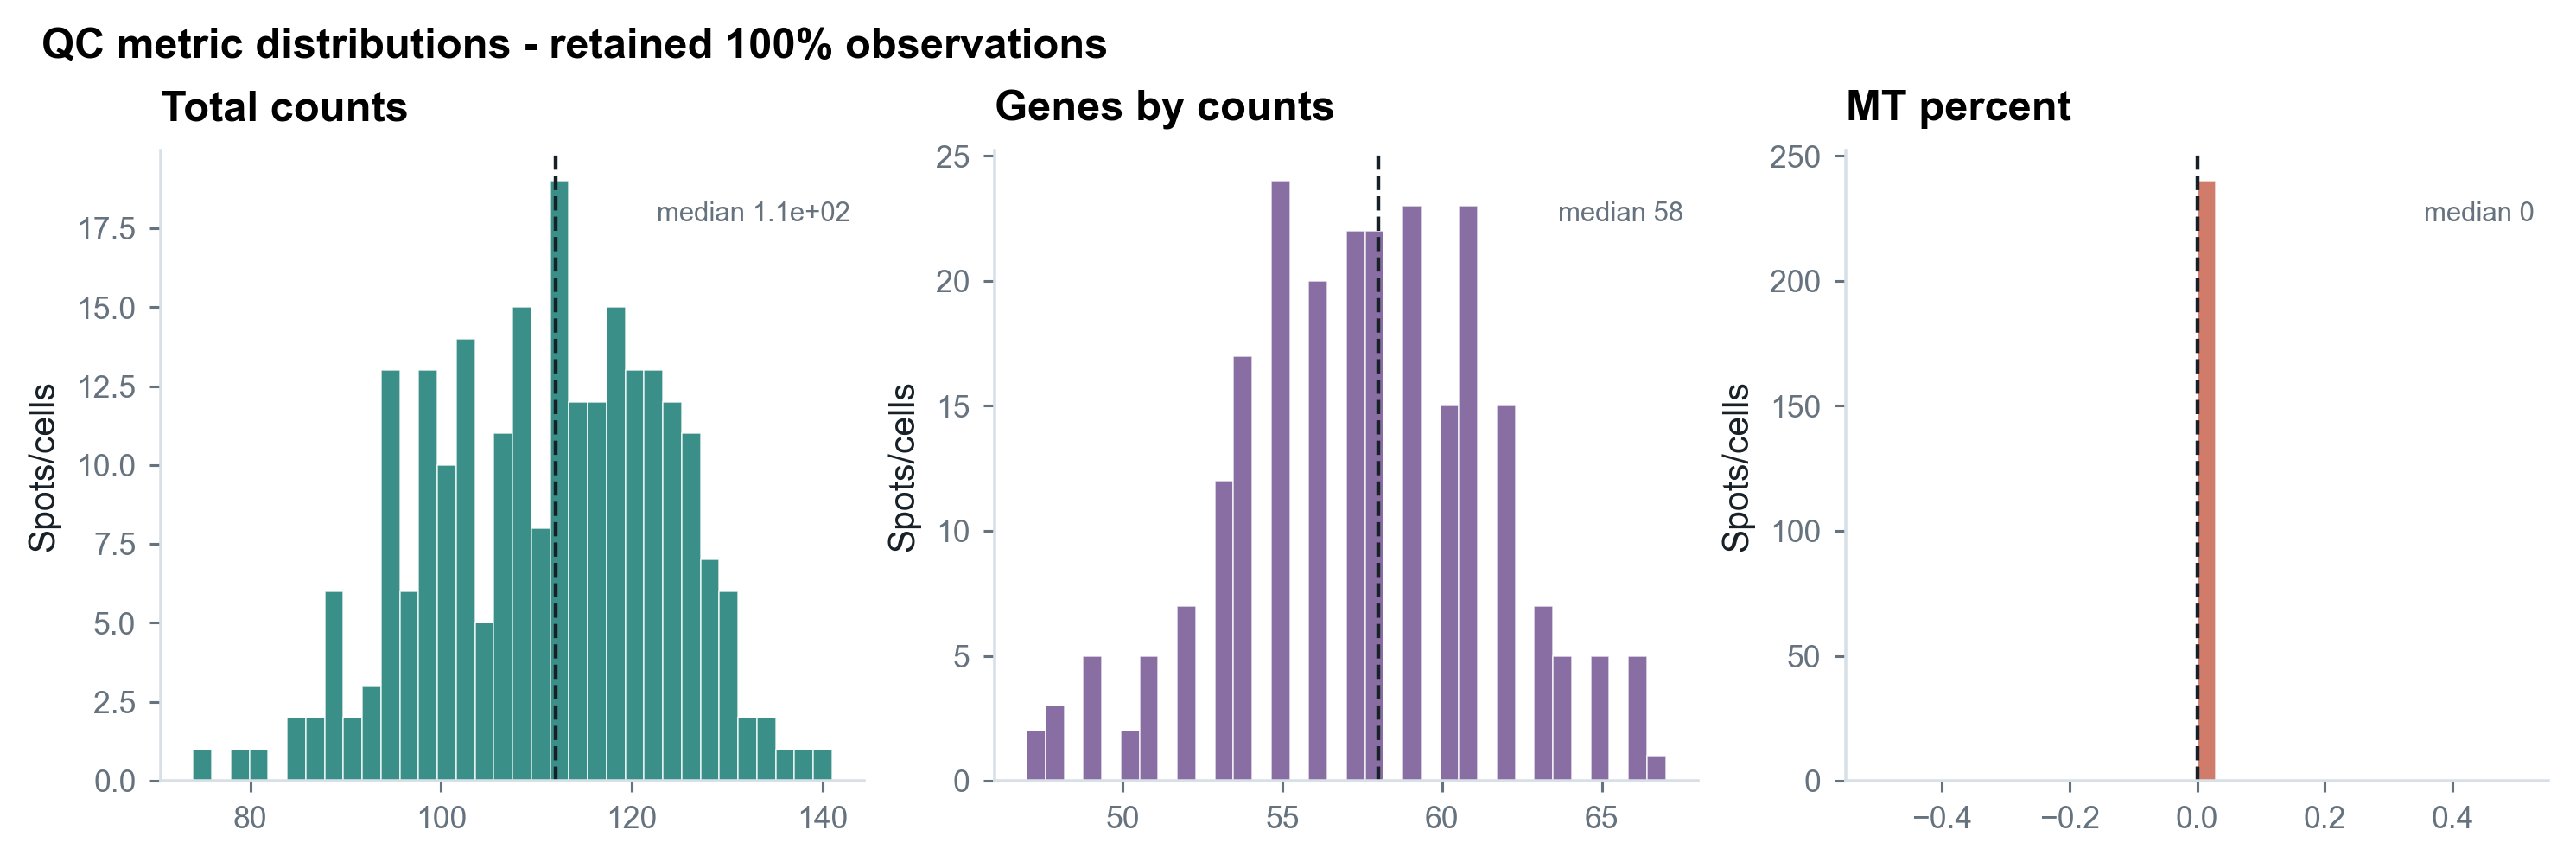
\includegraphics[width=\linewidth]{assets/demo_qc_metrics.png}
  \caption{QC 指标分布。}
\end{subfigure}
\hfill
\begin{subfigure}{0.49\textwidth}
  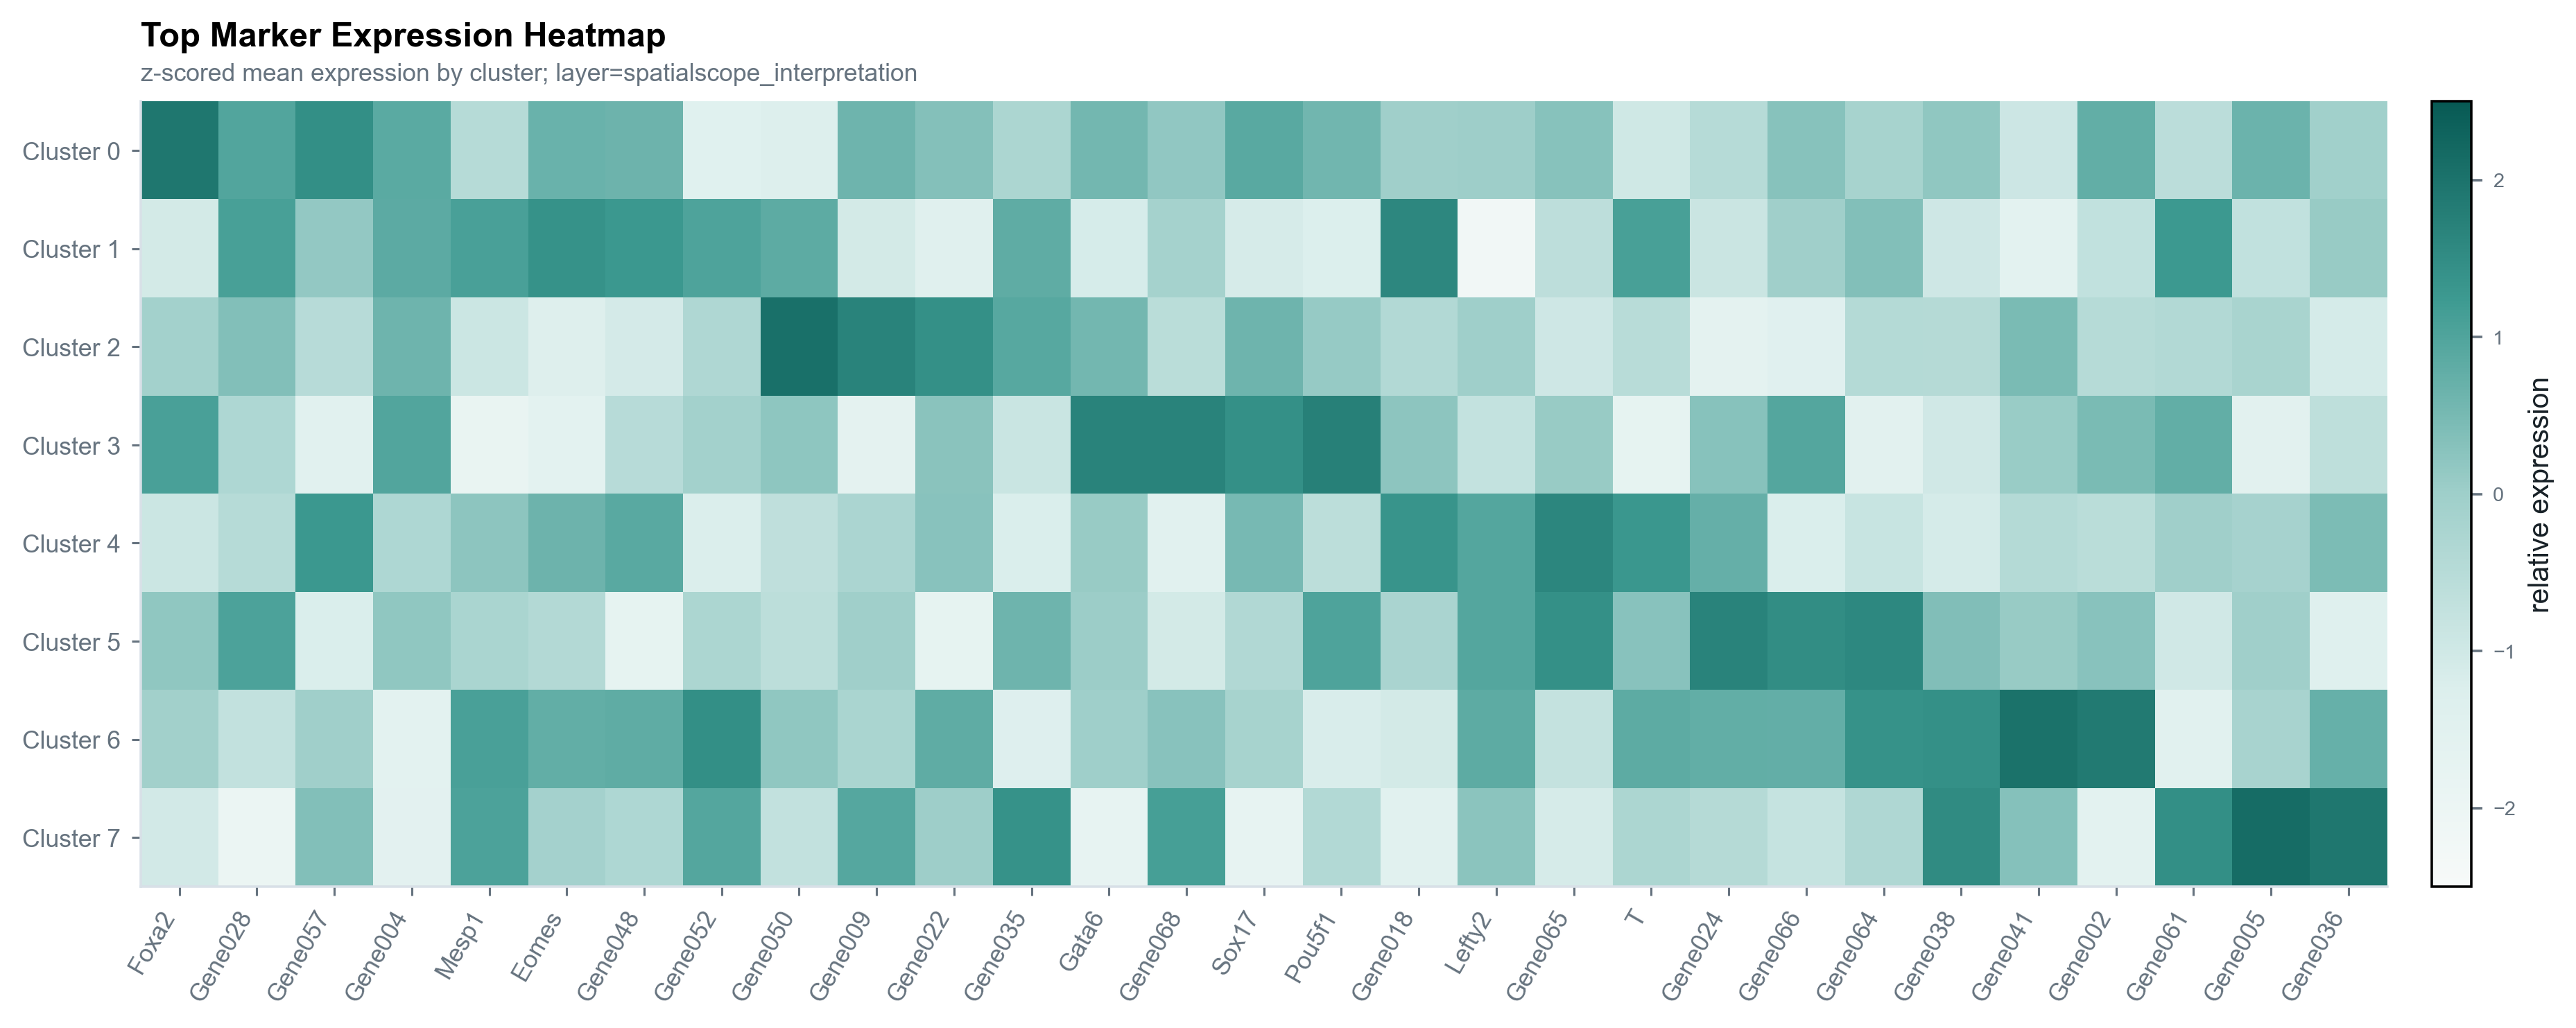
\includegraphics[width=\linewidth]{assets/demo_marker_heatmap.png}
  \caption{Top marker expression heatmap。}
\end{subfigure}
\caption{demo run 的质量控制与 marker gene 证据。}
\label{fig:demo-qc-marker}
\end{figure}

\subsection{线上部署验收}

提交前已对公开 Streamlit app 做浏览器端完整验收：

\begin{itemize}
  \item 线上 URL 正常打开，页面显示 \code{LLM active}。
  \item 选择 \code{demo_embryo.h5ad} 后，系统正确显示 240 spots、80 genes、spatial available、count-like。
  \item 输入中文研究问题后，系统生成 7 步分析方案。
  \item 点击批准运行后，Run 页面实时显示 LangGraph events。
  \item 运行完成后显示 10 events、6 figures、4 tables，并生成 \code{report.html}。
  \item Explore 页面展示 Spatial + UMAP、gene controls、evidence ID 和 Copilot 区域。
  \item Report 页面自动载入最新 run，显示 5 条 findings、evidence IDs、caveats 和 primary visual evidence。
  \item 浏览器 console 未发现 error 或 warning。
\end{itemize}

\section{真实数据验证：GSE278603 E7.5 mouse embryo}

课程推荐使用 ``Digital reconstruction of full embryos during early mouse organogenesis'' 对应的 GSE278603。
本项目提供 \code{scripts/download_real_demo.sh} 下载脚本，从 GEO 官方补充文件中提取
\code{GSM9046244_Embryo_E7.5_stereo_rep2.h5ad}。该文件约 31 MB，适合课程项目 smoke test。

\begin{table}[H]
\centering
\caption{真实数据 quick run 摘要。}
\begin{tabularx}{\textwidth}{L{0.28\textwidth}Y}
\toprule
项目 & 数值 \\
\midrule
Run ID & \code{20260625_154218_200361_fb6b32} \\
数据来源 & NCBI GEO GSE278603，E7.5 mouse embryo Stereo-seq sample \\
数据规模 & 8190 spots，16364 genes \\
空间坐标 & \code{obsm["X_spatial"]} 与标准化后的 \code{obsm["spatial"]} 可用 \\
矩阵状态 & log-normalized；系统建议使用 raw 作为安全表达来源 \\
QC 后规模 & 8190 spots，13844 genes \\
聚类结果 & 7 个 Leiden clusters \\
产物 & 5 figures，2 tables，9 trace events，0 warnings，0 errors \\
\bottomrule
\end{tabularx}
\end{table}

\begin{figure}[H]
\centering
\begin{subfigure}{0.49\textwidth}
  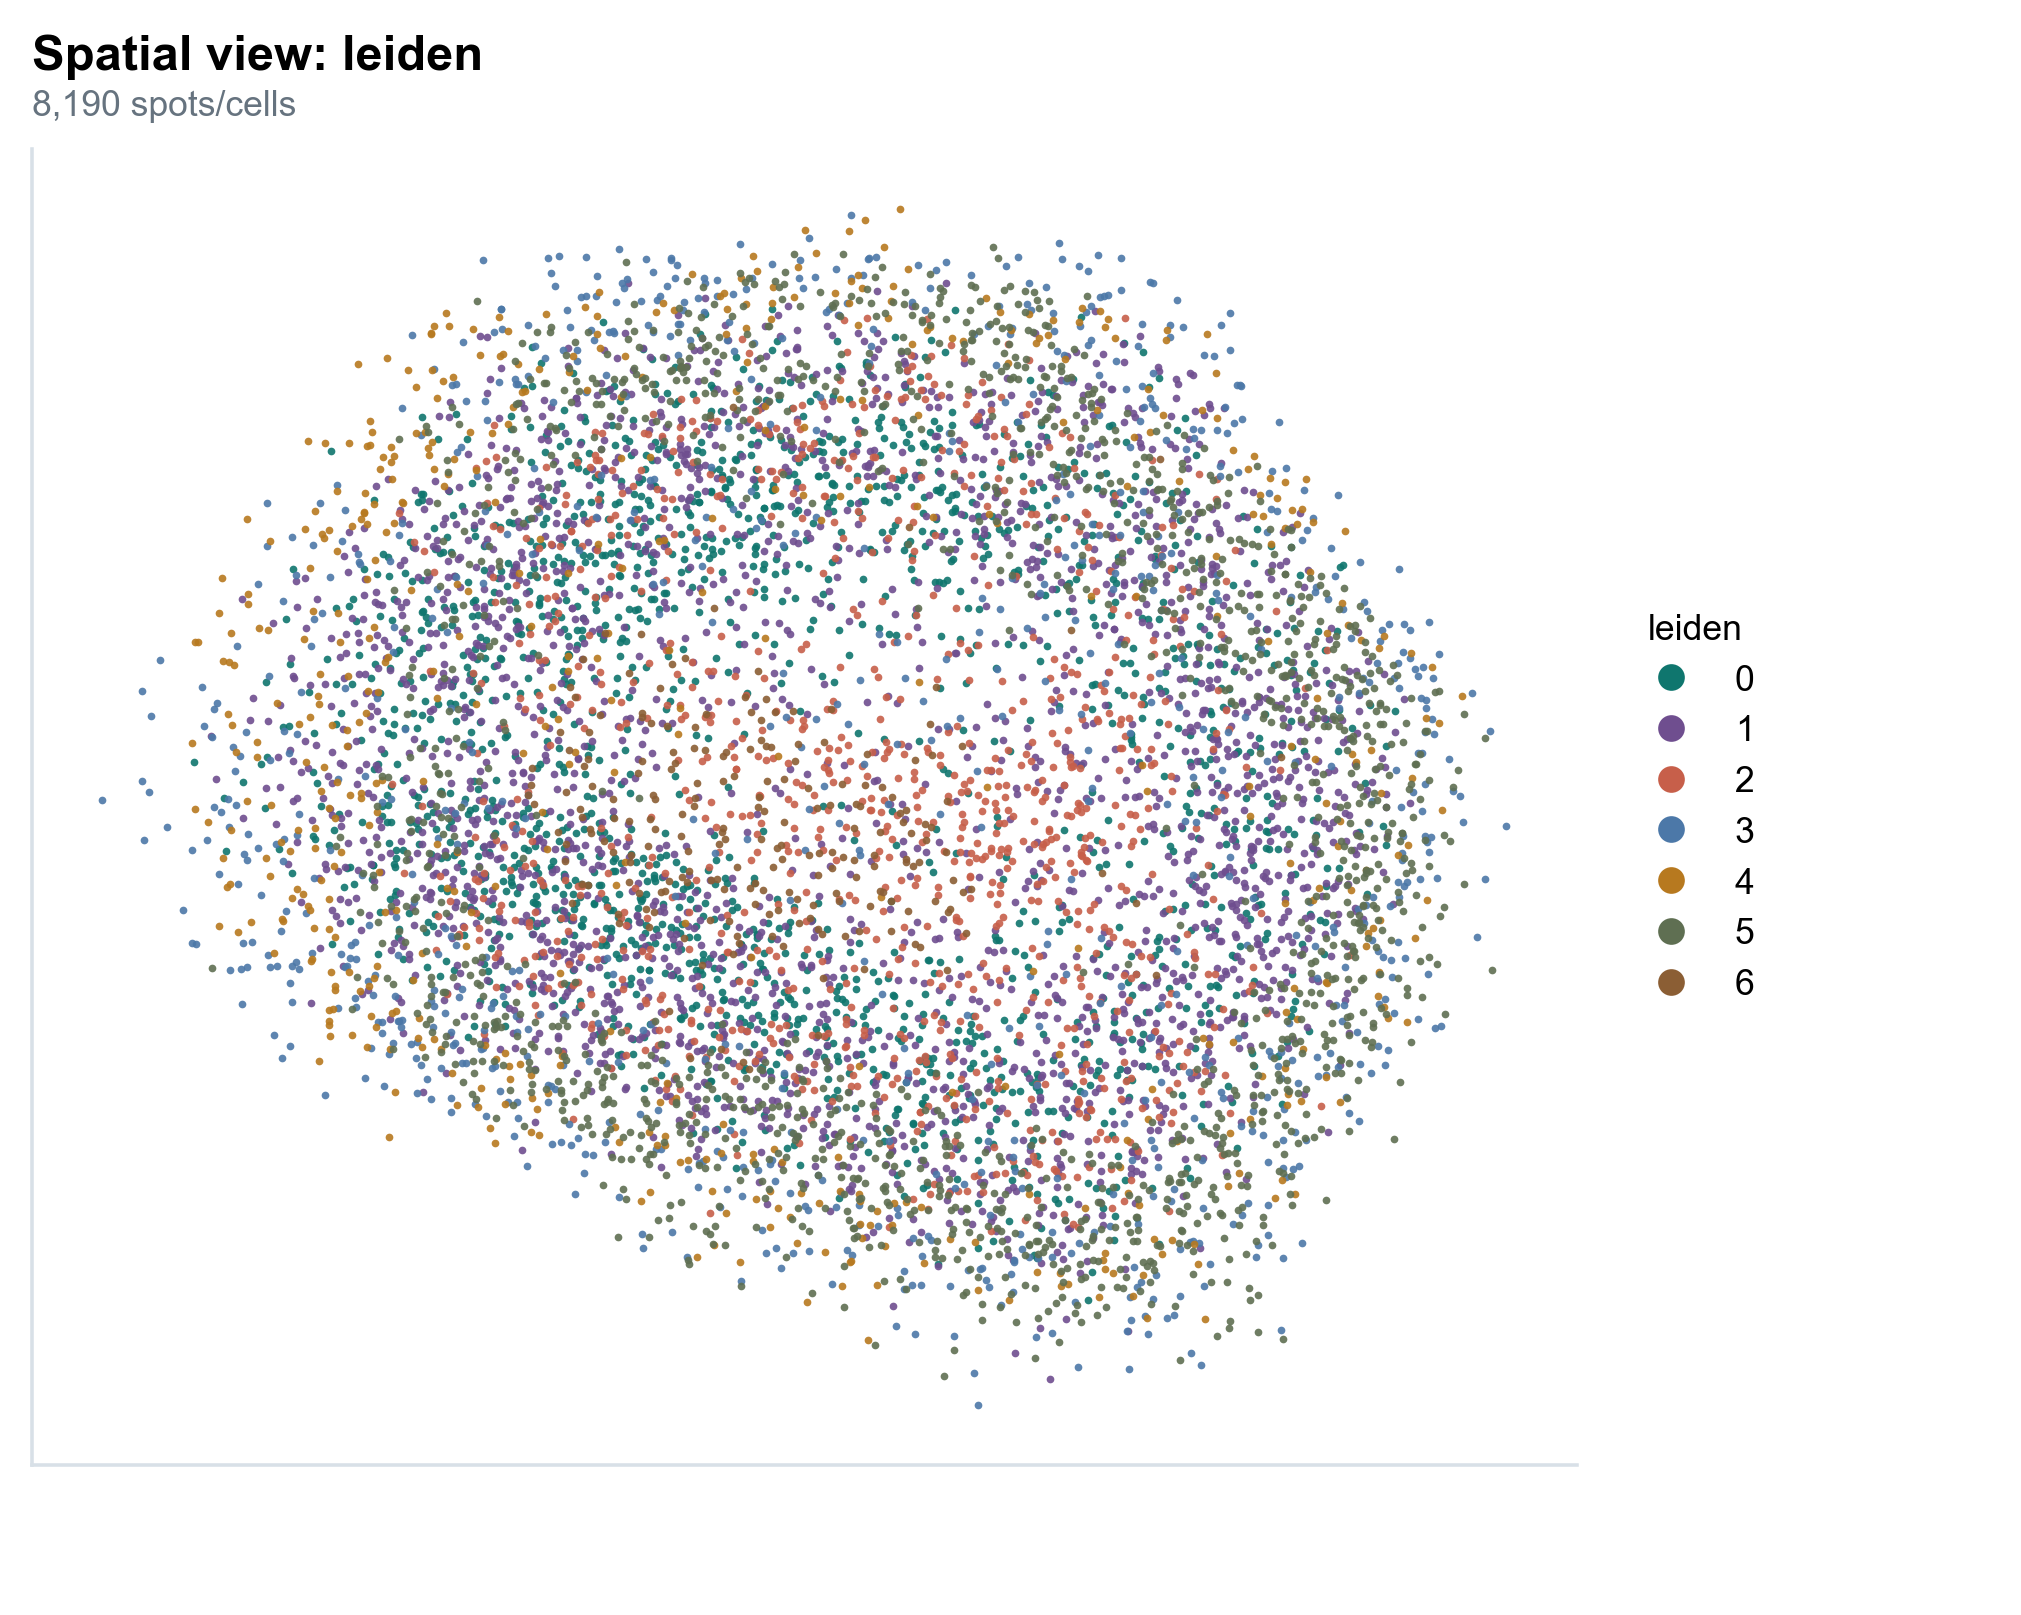
\includegraphics[width=\linewidth]{assets/real_spatial_leiden.png}
  \caption{真实 E7.5 样本中的 spatial Leiden clusters。}
\end{subfigure}
\hfill
\begin{subfigure}{0.49\textwidth}
  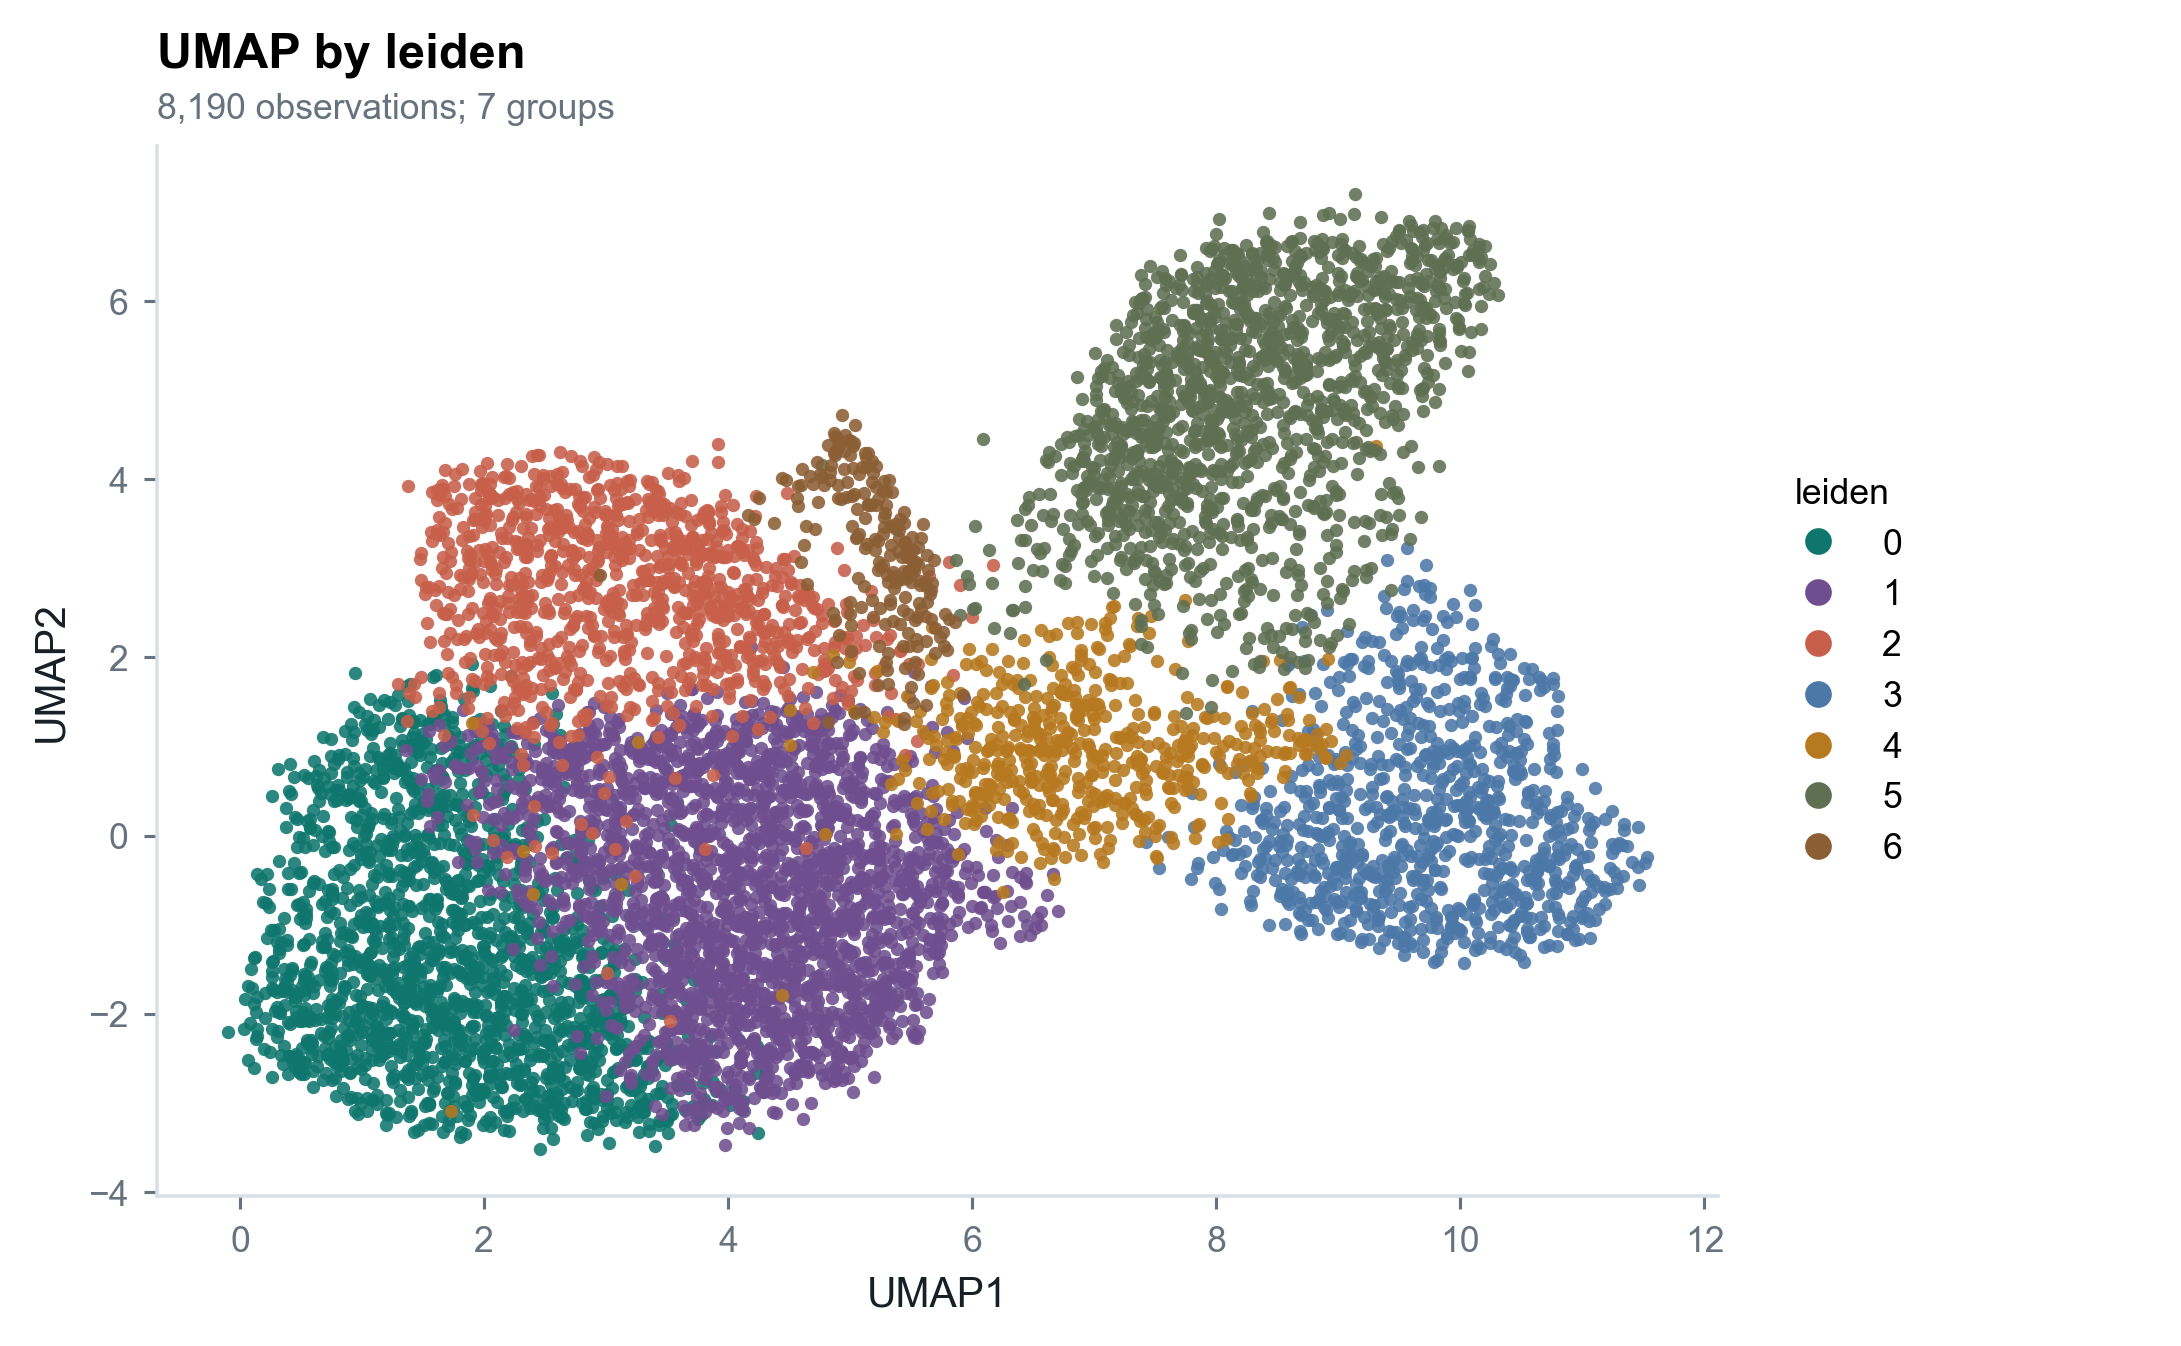
\includegraphics[width=\linewidth]{assets/real_umap_leiden.png}
  \caption{真实 E7.5 样本中的 UMAP cluster structure。}
\end{subfigure}
\caption{真实 GSE278603 样本 quick run 的空间结构和表达空间结构。}
\label{fig:real-cluster}
\end{figure}

\begin{figure}[H]
\centering
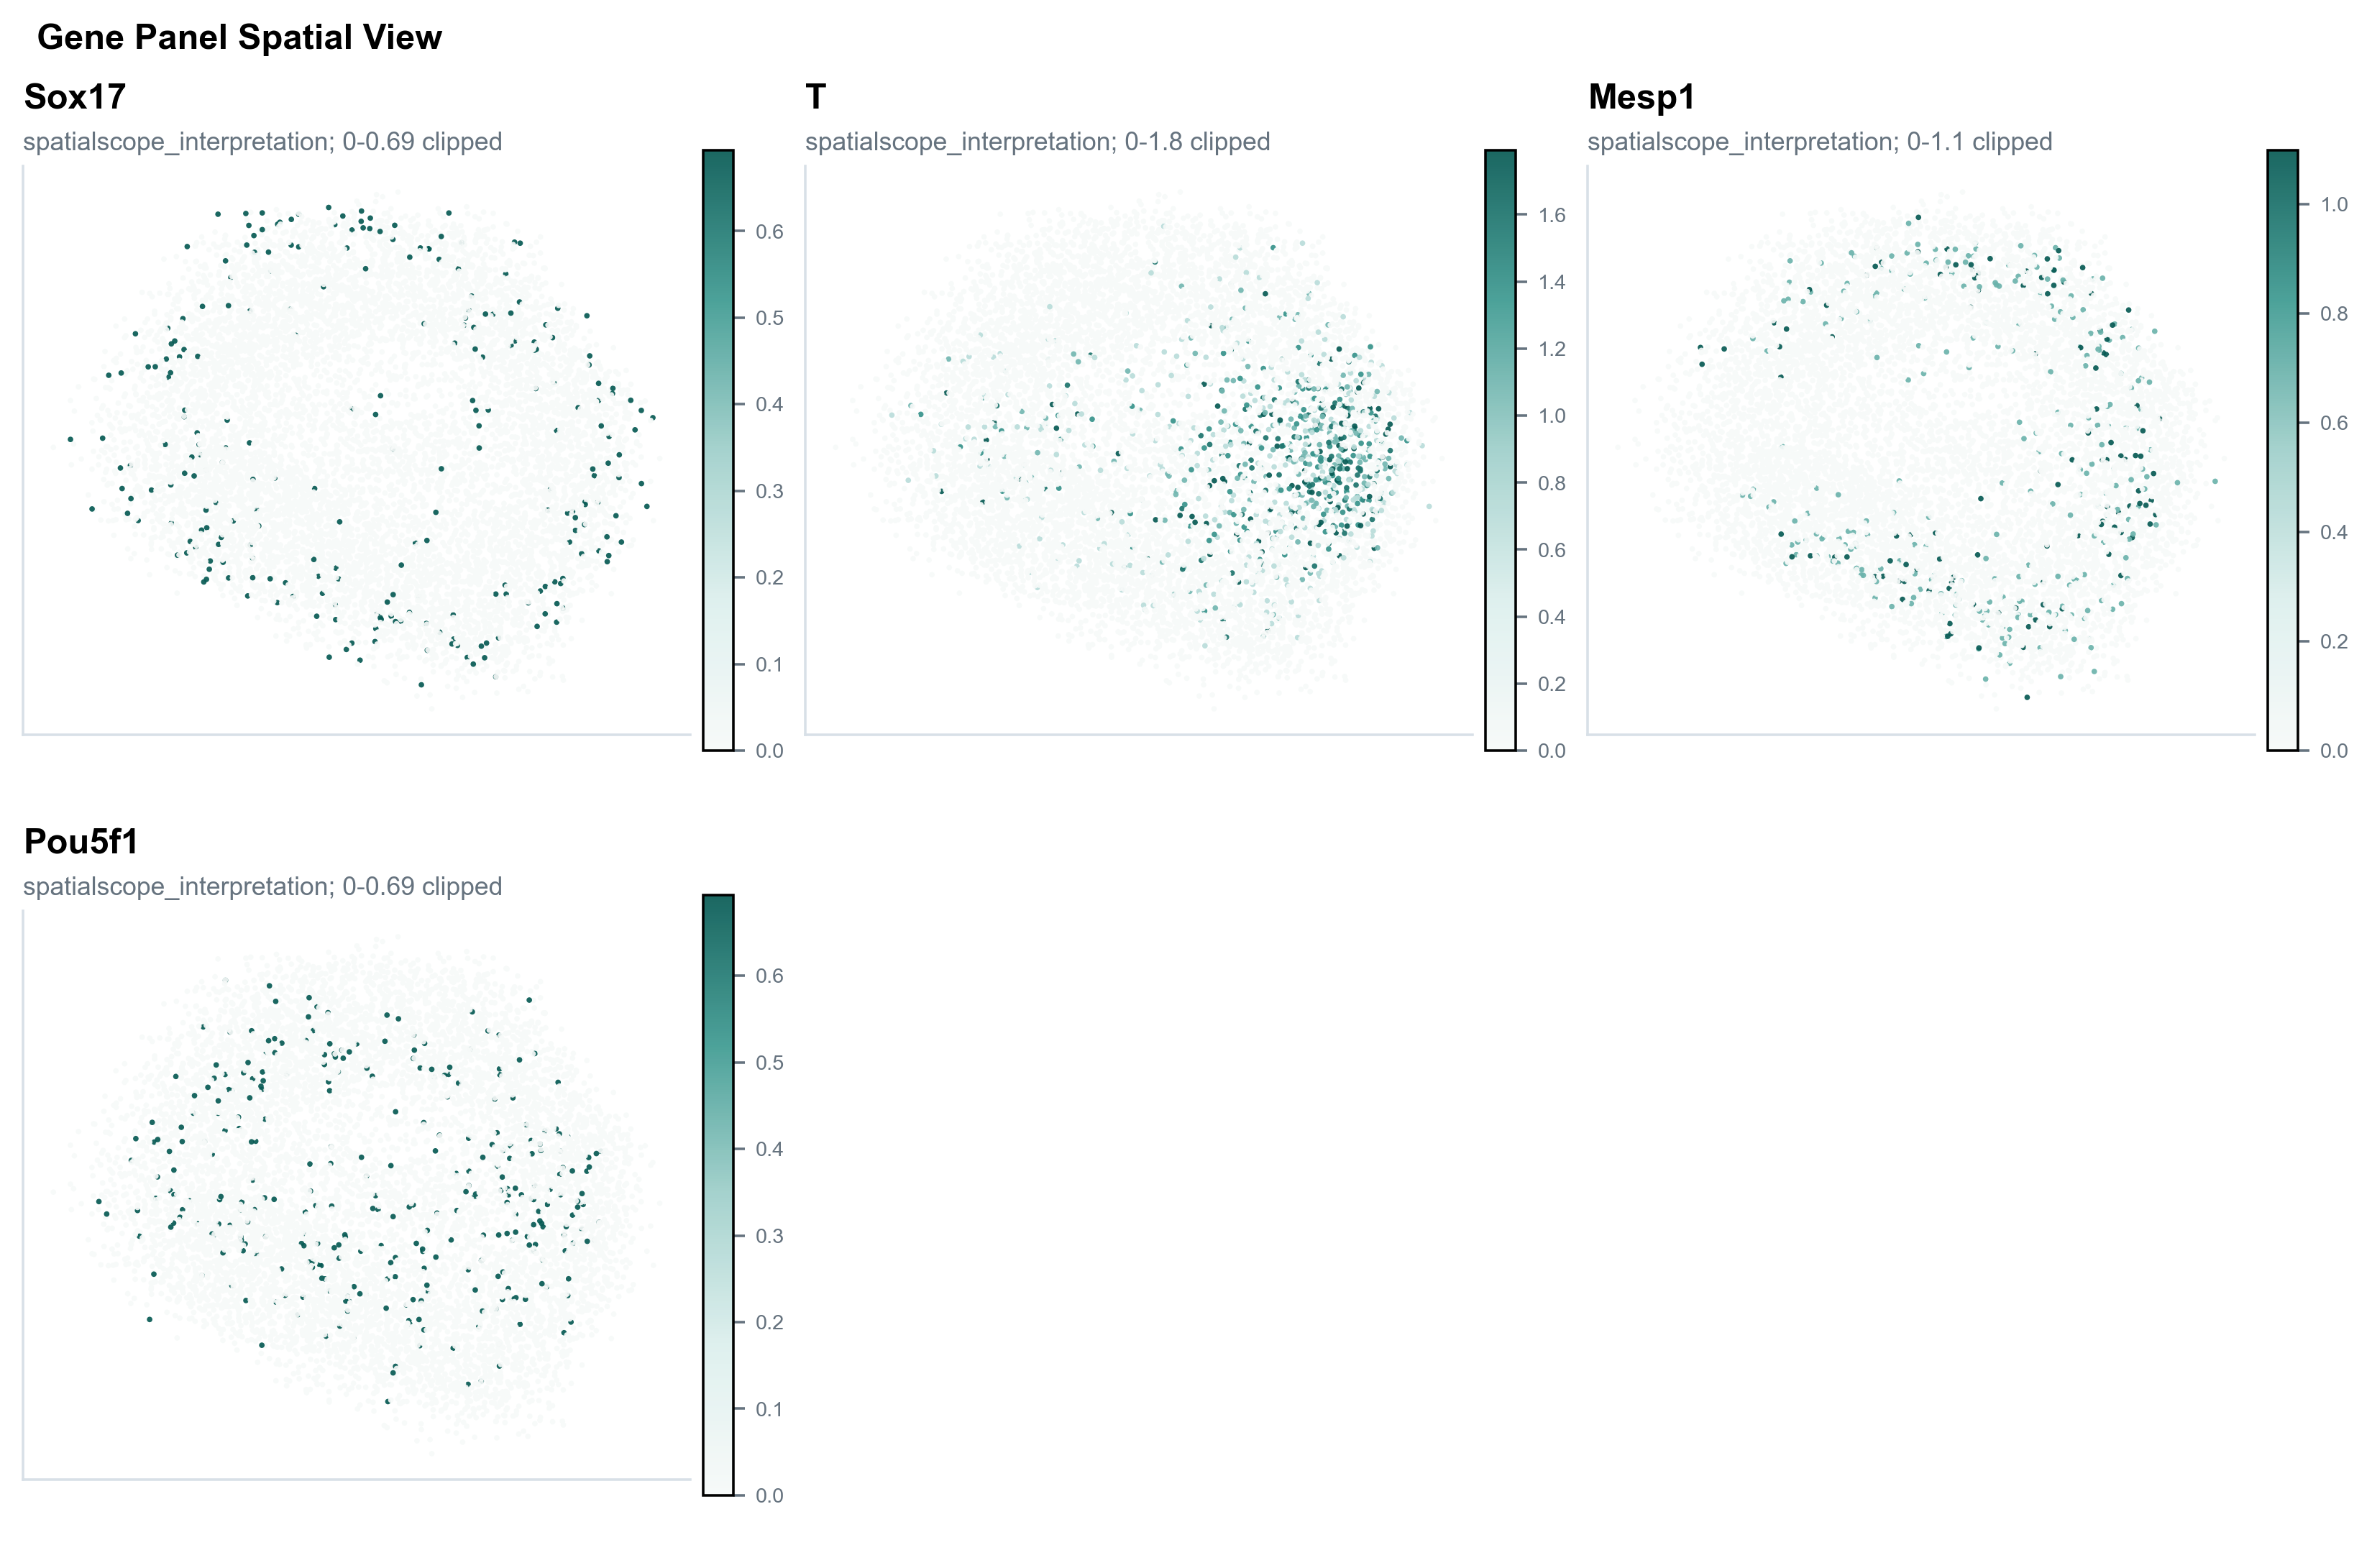
\includegraphics[width=0.96\textwidth]{assets/real_gene_panel.png}
\caption{真实样本中 Sox17、T、Mesp1、Pou5f1 的空间表达 quick panel。该结果用于验证工具链可处理真实 Stereo-seq AnnData，不作为完整生物学结论。}
\label{fig:real-gene-panel}
\end{figure}

真实数据验证具有两方面意义。第一，系统并未依赖 synthetic demo 的固定字段，能够识别真实数据中的
\code{X_spatial} 坐标并标准化为 \code{spatial}。第二，真实数据暴露了更复杂的表达来源问题：矩阵
被判断为 log-normalized，系统需要优先选择 raw 或安全 interpretation layer，而不能直接将当前
\code{X} 视为 counts 进行解释。

\section{可复现性、测试与 GitHub 管理}

\subsection{测试}

项目包含单元测试、数据测试、CLI smoke test 和浏览器端手工验收。提交前的关键结果为：

\begin{itemize}
  \item \code{pytest -q}: 99 passed。
  \item CLI demo smoke run：成功生成 \code{report.html}，0 warnings，0 errors。
  \item 真实数据 quick run：成功生成 \code{report.html}，0 warnings，0 errors。
  \item GitHub Actions CI：成功运行测试和 demo smoke command。
  \item 线上 Streamlit：完整流程验证通过。
\end{itemize}

\subsection{输出包}

每次运行会写入 \code{outputs/runs/<run_id>/}，包括：

\begin{itemize}
  \item \code{report.html}: 面向用户的 Research Brief；
  \item \code{run_metadata.json}: 参数、环境、产物和质量信息；
  \item \code{agent_trace.json}: 工具执行 trace；
  \item \code{parameters.yaml}: 关键参数；
  \item \code{figures/} 与 \code{tables/}: 图表产物；
  \item \code{DATASET_CARD.md}: 数据规模、schema preview 和隐私边界；
  \item \code{RERUN.md} 与 \code{rerun.sh}: 复跑说明；
  \item \code{run_bundle.zip}: 便携式交付包。
\end{itemize}

\subsection{GitHub 项目规范}

仓库已经包含标准开源项目结构，包括 \breakcode{README.md}、\breakcode{environment.yml}、
\breakcode{pyproject.toml}、\breakcode{.env.example}、\breakcode{LICENSE}、
\breakcode{SECURITY.md}、\breakcode{CITATION.cff}、\breakcode{CHANGELOG.md}、issue template、
PR template、Dependabot、GitHub Actions CI 和 GitHub Pages。大型 \breakcode{.h5ad} 文件和
\breakcode{outputs/runs/} 被 \breakcode{.gitignore} 排除，避免把数据和运行产物误提交到公开仓库。

\section{创新性与扩展性}

与固定 Scanpy notebook 相比，本项目的扩展设计主要体现在以下几个方面：

\begin{enumerate}
  \item \textbf{Agent 化的空间组学流程。} 使用 LangGraph 显式建模节点、状态、条件边和 repair loop，
  让分析过程可解释、可中断、可恢复。
  \item \textbf{证据约束的 LLM。} LLM 只围绕 evidence pack 解释，不接触完整矩阵，并显示 exact
  evidence IDs，使每条结论都能回到具体图、表或统计摘要。
  \item \textbf{结构化 prompt 与 schema 校验。} 任务解析、计划生成、修复建议、finding 合成和
  Copilot 回答均使用 JSON schema 与 Pydantic validation，避免把自由文本直接交给执行器。
  \item \textbf{Human-in-the-loop。} 分析方案需要用户审阅批准，Report finding 也提供人工 review 入口。
  \item \textbf{表达层安全机制。} 在 marker/gene interpretation 前检查 count-like、log-normalized、scaled
  或 unknown matrix state，避免错误表达来源带来的伪结论。
  \item \textbf{面向研究流程的交互界面。} 主界面围绕 Project、Run、Explore、Report 组织，保留必要英文术语，
  并通过 logo、Acknowledgements 和 Copilot 入口形成一致的视觉识别。
  \item \textbf{真实数据可验证。} 提供 GSE278603 下载脚本和真实 E7.5 样本 quick run，降低对 toy data 的依赖。
\end{enumerate}

\section{不足与展望}

本项目已经覆盖课程核心要求，但仍有明确边界：

\begin{itemize}
  \item 在线 demo 为了稳定性使用 synthetic embryo dataset；真实数据建议本地运行，在线大数据受 Streamlit Cloud
  内存和启动时间限制。
  \item marker gene ranking 只是候选差异表达线索，不等同于细胞类型注释或发育机制证明。
  \item SVG 与 neighborhood enrichment 依赖 Squidpy 扩展环境，当前以可选工具和 graceful fallback 形式存在。
  \item 细胞通讯、Tangram、cell2location、STAGATE/GraphST 等高级方法尚未进入 v1 主流程。
  \item LLM 解释质量依赖 evidence pack 的组织方式，仍需要人工生物学审阅。
\end{itemize}

未来可以继续扩展：引入更系统的空间可变基因统计、多 run 对比、marker ontology 映射、细胞类型注释建议、
PDF/Word 自动报告导出，以及面向真实大型数据的远程计算后端。

\section{总结}

SpatialScope Agent 根据课程任务完成了一个可运行、可部署、可复核的空间转录组分析系统。系统不仅覆盖
\code{.h5ad} 读取、质量控制、预处理、降维聚类、空间可视化和 marker gene 分析等基础功能，还将
Agent 的状态、工具、计划、循环、修复和解释机制整合到浏览器端流程中。

从系统完整性看，项目已包含 GitHub 仓库、环境配置、测试、在线部署、真实数据 smoke run、最终报告和
课堂 demo script。从科学可靠性看，系统对表达层安全、证据编号、局限性说明和 LLM 边界进行了显式约束。
后续课堂展示可重点说明 Agent 如何先理解数据、再制定计划、再生成证据，并在证据边界内进行解释。

\section*{Acknowledgements}
\addcontentsline{toc}{section}{Acknowledgements}

\begin{summarybox}{Acknowledgements}
  \begin{minipage}{0.13\textwidth}
    \centering
    
\includegraphics[width=1.25cm]{assets/logo.png}
  \end{minipage}
  \hfill
  \begin{minipage}{0.82\textwidth}
    We gratefully acknowledge Professor Peng Xie from the School of Biological Science and Medical Engineering,
    Southeast University. We also thank Teaching Assistant Binyu Gao for guidance and support throughout the course project.
  \end{minipage}
\end{summarybox}

\section*{参考资料}
\addcontentsline{toc}{section}{参考资料}

\begin{enumerate}
  \item Wolf, F. A., Angerer, P., and Theis, F. J. Scanpy: large-scale single-cell gene expression data analysis.
  \textit{Genome Biology} 19, 15 (2018).
  \item Palla, G. et al. Squidpy: a scalable framework for spatial omics analysis. \textit{Nature Methods} 19, 171-178 (2022).
  \item AnnData documentation. \url{https://anndata.readthedocs.io/}
  \item Scanpy documentation. \url{https://scanpy.readthedocs.io/}
  \item Squidpy documentation. \url{https://squidpy.readthedocs.io/}
  \item LangGraph documentation. \url{https://langchain-ai.github.io/langgraph/}
  \item Streamlit documentation. \url{https://docs.streamlit.io/}
  \item NCBI GEO GSE278603. \url{https://www.ncbi.nlm.nih.gov/geo/query/acc.cgi?acc=GSE278603}
  \item Digital reconstruction of full embryos during early mouse organogenesis. \textit{Cell} (2025).
  DOI: \url{https://doi.org/10.1016/j.cell.2025.05.035}
\end{enumerate}

\end{document}
